% --------------------------------------------
%		CAPITOLO 5
%---------------------------------------------

\chapter{TJ-Monopix2 characterization} \label{ch:TJ2}

In this chapter we will go through the main features of TJ-Monopix2 designed to address efficiency degradation after irradiation, one of the main issues of its predecessor TJ-Monopix1 (\autoref{sec:TJ}). The characterization of the chip is crucial in the VTX upgrade program and in the design of the next OBELIX chip.\\
The chip W14R12, shown in~\autoref{fig:w14r12}, is one of the sensors tested during the first Test Beam (TB) campaign in Desy (June 2022). It has been fully characterized in Pisa and in particular several aspects have been analyzed, among which:

\begin{enumerate}
\item TOT calibration by internal charge injection;
\item characterization with radioactive sources and absolute calibration;
\item systematic study of different registers' settings to operate the chip at low threshold;
\item investigation of an important issue with cross-talk, due to digital signal from the readout, discovered trying to operate the matrix at low threshold (below 250~$e^{-}$).
\end{enumerate}

This detailed characterization returned crucial results (points 1, 2 above) for the Test Beam data reconstruction and the simulations of the upgraded VTX detector with CMOS MAPS devices. Furthermore the optimization of the registers to reduce the operating threshold was very useful for the preparation of the next TB (July 2023) campaign with irradiated sensors.


%FOTO TJ MONOPIX 2
\begin{figure}[h!]
\centering
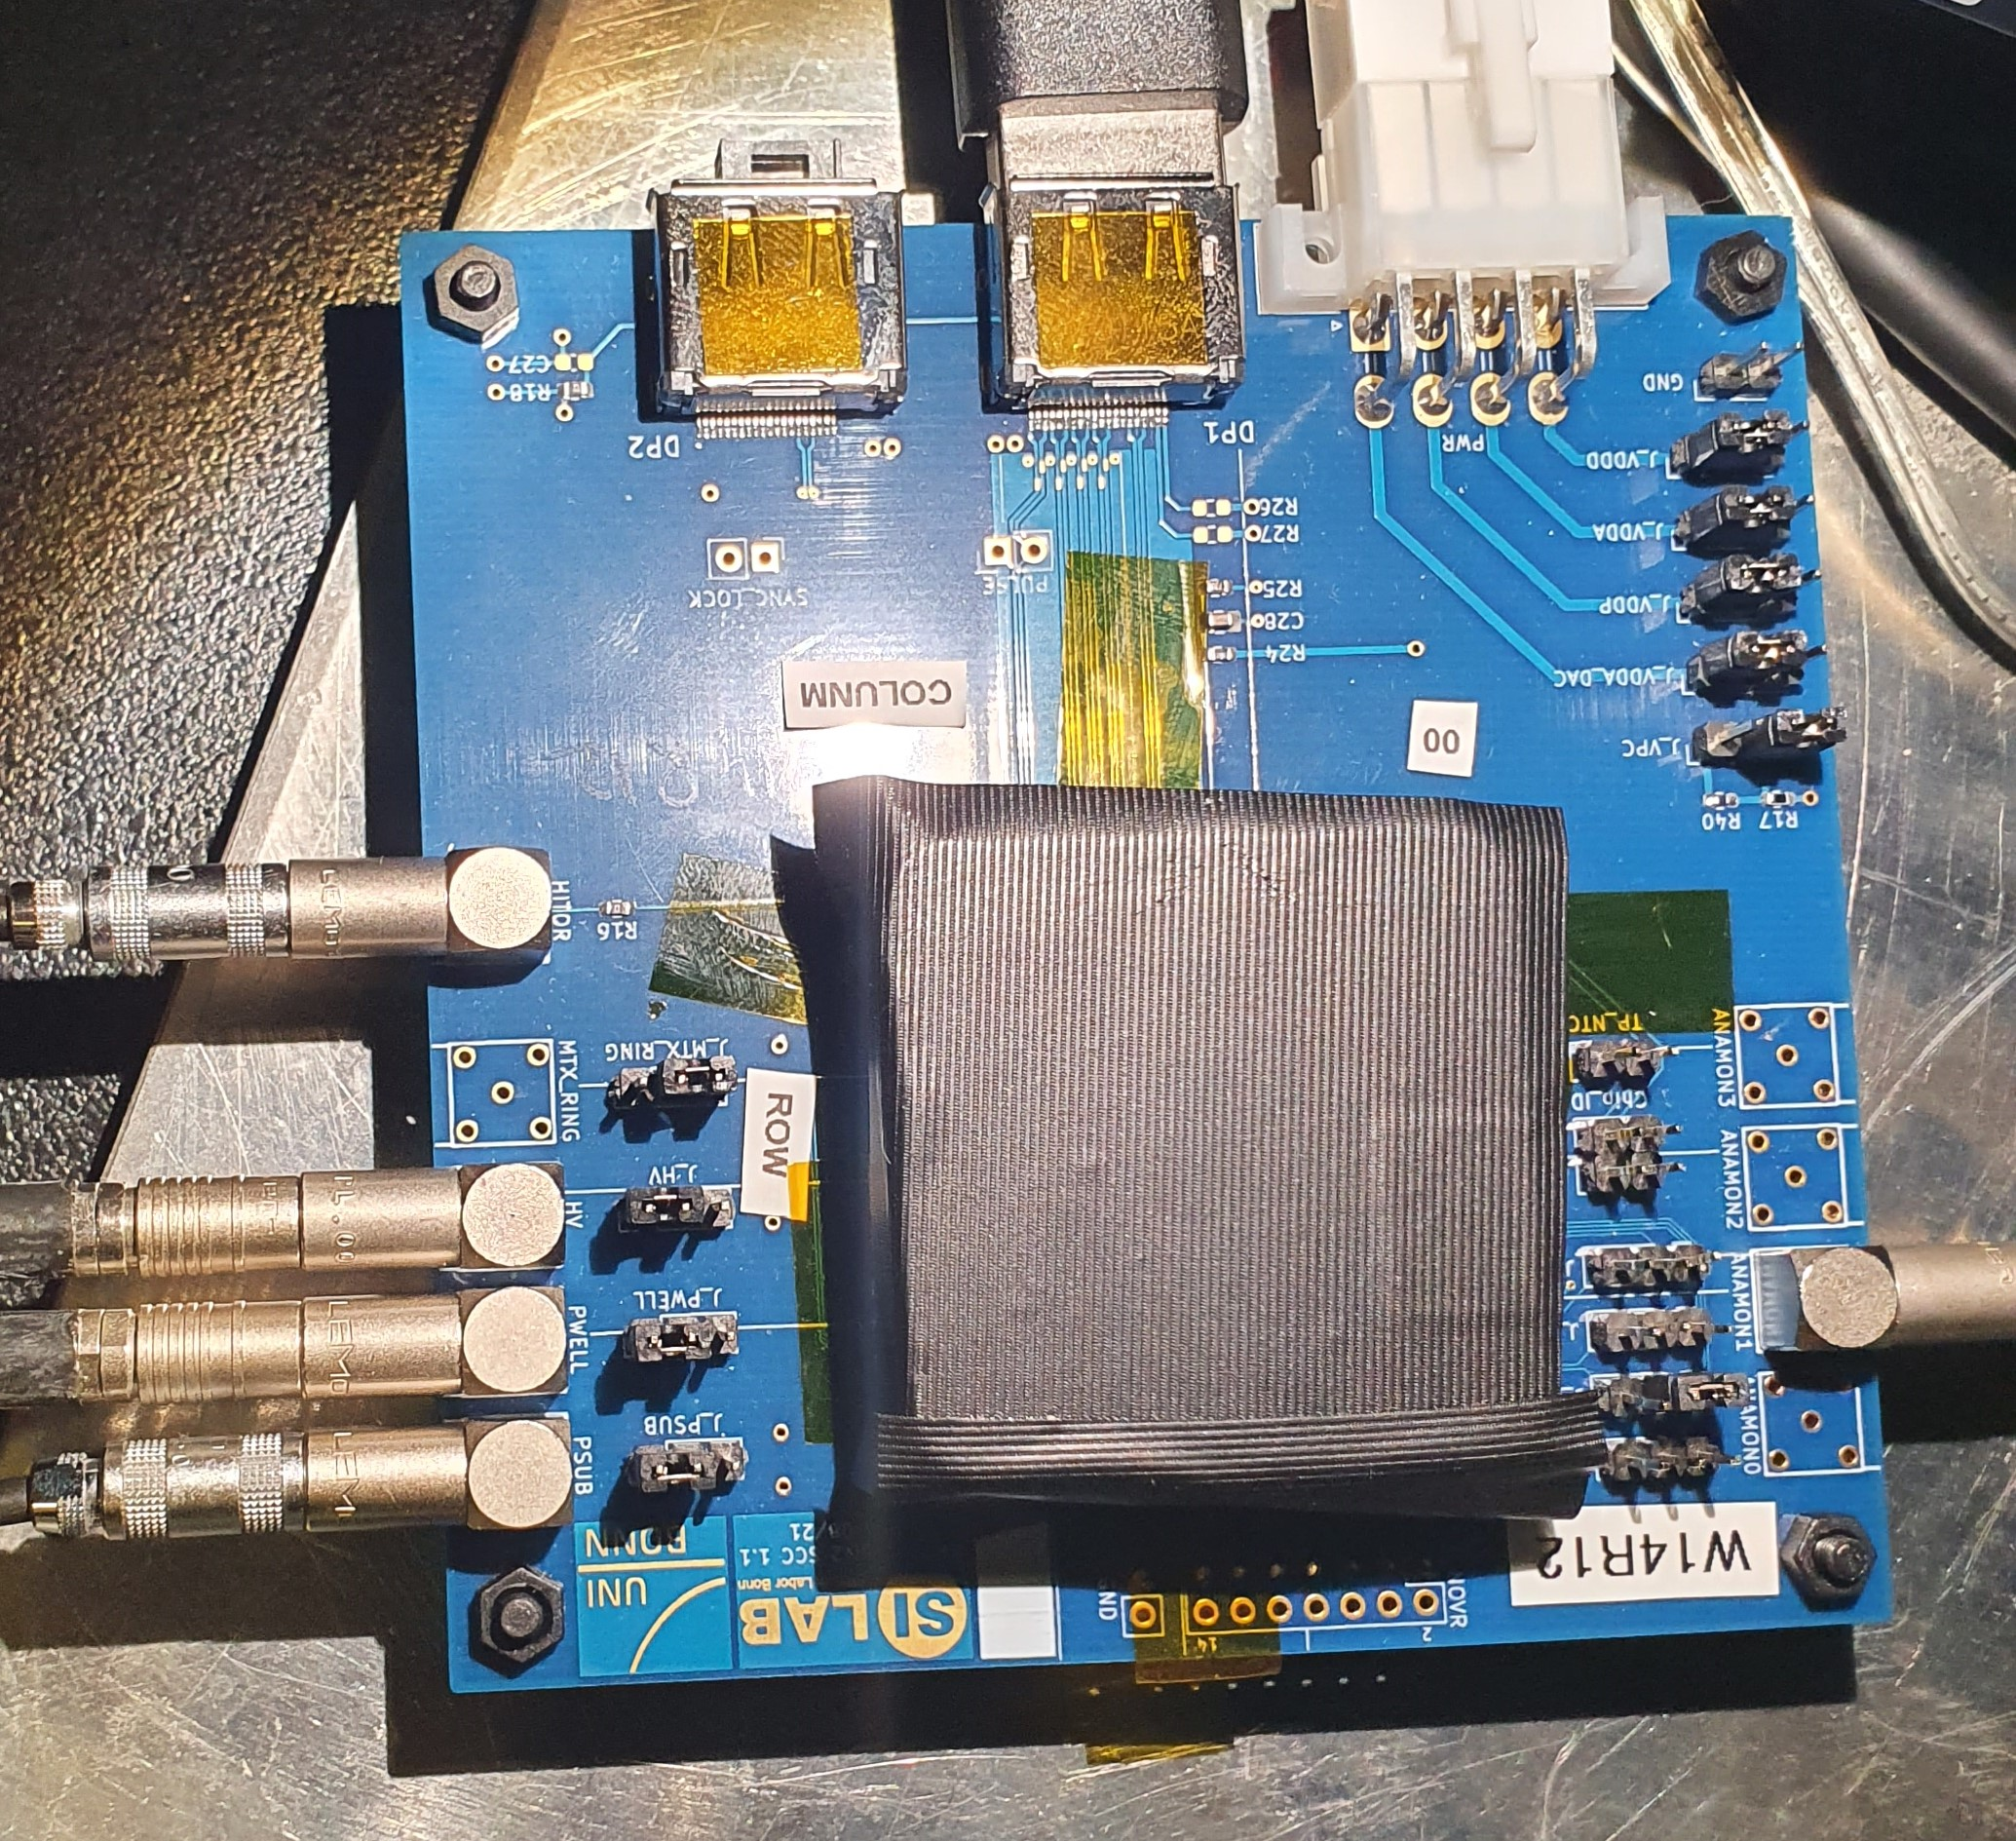
\includegraphics[scale=.08]{W14R12}
\caption{The W14R12 chip tested during the Test Beam in Desy.}
\label{fig:w14r12}
\end{figure}


% --------------------------------------------
%	5.1 MATRIX AND FLAVORS
%---------------------------------------------

\section{Matrix and flavors}


TJ-Monopix2 is a small collection electrode DMAPS prototype in TowerJazz \SI{180}{nm} process. The need to create a sensor capable to maintain high efficiency even after irradiation, required improvements compared to TJ-Monopix1 in two important fields: a lower operating threshold,  to keep a good efficiency with the reduced charge collected after irradiation, and a smaller pixel pitch, to increase charge collection efficiency all over its area, especially in the corners.\\

To achieve these goals, a different in-pixel front-end circuit was implemented and many efforts were focused on the pixel layout optimization to reduce its size, which was decreased from \numproduct{36 x 40}~\unit{\micro m^{2}} in TJ-Monopix1 to \numproduct{33.04 x 33.04}~\unit{\micro m^{2}} (pixel pitch). The pixel dimensions are critical to accomplish faster charge collection across all active area, increasing the lateral electric field (\autoref{sec:TJ}) \cite{Munker_2019}. For this reason it was necessary a special effort to design and create a smaller pixel pitch but still adequate to embody the full digital readout. All this required to work at the technology density limit and to optimize the circuit design.

In order to operate with a lower threshold, TJ-Monopix2 incorporates an improved front-end circuit that reduces the noise by $\approx$ 40\% and the threshold dispersion by about 80-90\% with respect to TJ-Monopix1. Furthermore, in-pixel threshold tuning has been integrated to achieve a more uniform threshold distribution across the pixel matrix, particularly after irradiation. As a result of these improvements, the operating threshold in optimized working conditions, was expected to be at $\approx$ 100~$e^{-}$, three times lower than in TJ-Monopix1, the noise less than 8~$e^{-}$, and the threshold dispersion less than 10~$e^{-}$ (\autoref{tab:tj2_spec}) \cite{Moustakas:2021gjr}. 

\medskip

\begin{table}[h!]
\centering
\begin{tabular}{c|c}
\hline
Specification & Value \\
\hline
\hline \\[-2.5ex]
Threshold & $\approx$ 100 $e^{-}$\\[0.5ex]
\hline
Noise & $\leq$ 8 $e^{-}$ \\ [0.5ex]
\hline
Threshold dispersion & $\leq$ 10 $e^{-}$\\[0.5ex]
\hline
\hline
\end{tabular}
\caption{Expected performance of TJ-Monopix2.}
\label{tab:tj2_spec}
\end{table}


%-----------------------------------------------------------------------------------------------

\subsection{Flavors} \label{sec:flavors}

The prototype is a \numproduct{2 x 2}~\unit{cm^{2}} pixel matrix, \SI{300}{\micro m} thick, and consisting of \numproduct{512 x 512} pixels. The total active area is approximately \SI{286}{mm^{2}}.


As shown in~\autoref{fig:tj2matrix}, the matrix is divided in four sectors, named \textit{flavors} that implement different variations of the front-end circuit. In the first two flavors the collection electrode is directly DC-coupled to the readout electronics;  the continuous baseline reset is implemented by a forward bias diode, but they differ in the pre-amplifier circuit design. The second flavor, named \textbf{Cascode FE}, includes an extra-cascode transistor that increases the pre-amplifier gain, which in turn leads to a 50\% reduction of the threshold dispersion compared to the first flavor, the \textbf{Normal FE}. The other two flavors consist of AC-coupled pixels (through a metal-oxide-metal MOM capacitor) and in particular, the \textbf{HV-Cascode FE} also incorporates the aforementioned pre-amplifier variation. AC-coupling allows to apply a high positive bias voltage (HV stands for High Voltage) to the collection electrode widening the depleted region, but at the same time causing signal losses mainly due to the additional parasitic capacitance introduced into the sensitive input node.\\


\begin{figure}[h!]
\centering
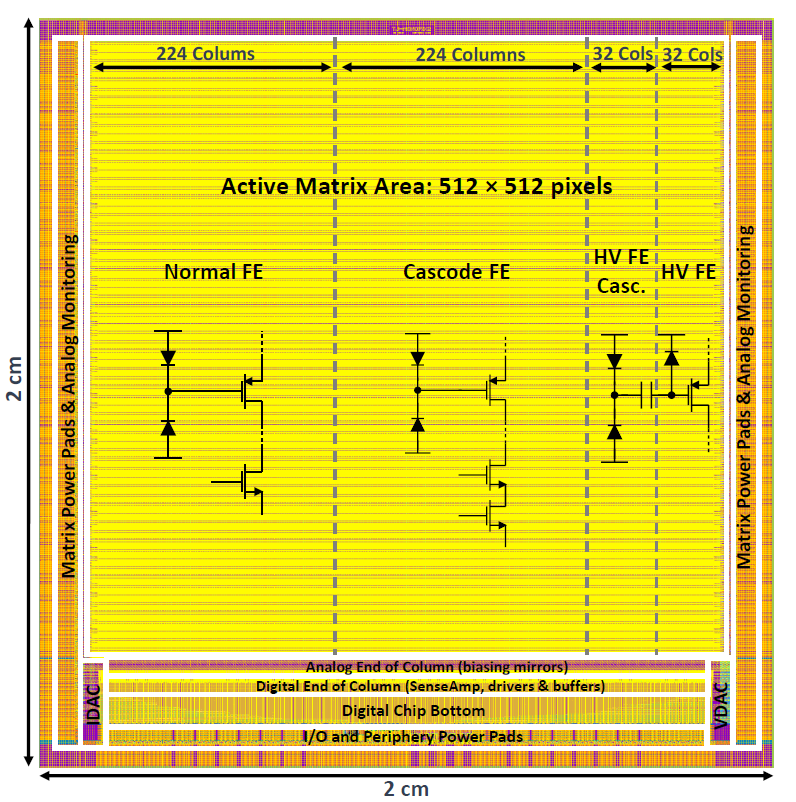
\includegraphics[scale=.5]{Matrix}
\caption{The layout of the TJ-Monopix2 prototype divided in four different flavors: Normal, Cascode, HV-Cascode and HV FE.}
\label{fig:tj2matrix}
\end{figure}


%-----------------------------------------------------------------------------------------------%

\subsection{Pixel design}\label{sec:improved_circuit}

The \numproduct{2 x 2} pixel core layout, shown in~\autoref{fig:tj2core}, is fully optimized and it is designed to share as much features as possible between the four pixels. The analog area incorporates the front-end circuit, the 3-bit threshold tuning DAC and the pixel configuration registers. The digital region is composed by the 7-bit Leading Edge (LE) and Trailing Edge (TE) memory (14 SRAM cells per pixel), the 10 bit address ROM (2 bit for the pixel position inside the core and 8 for the group address) and the readout control logic. 

\begin{figure}[h!]
\centering
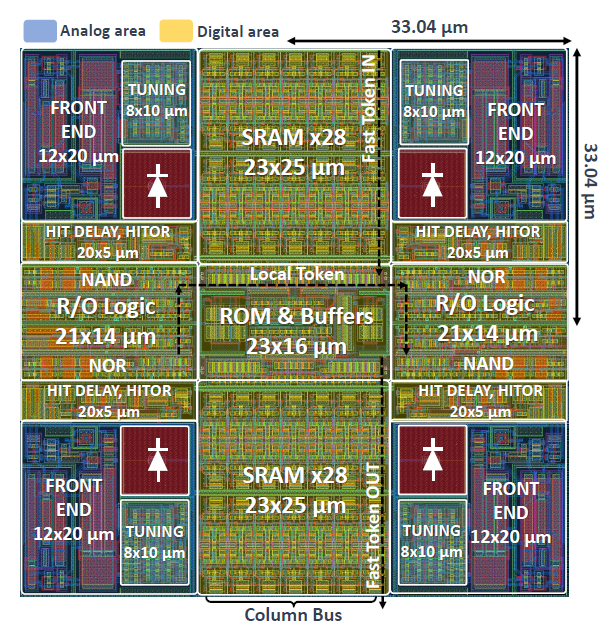
\includegraphics[scale=.55]{pixel_core}
\caption{Layout of a TJ-Monopix2 \numproduct{2 x 2} pixel core. In blue the analog area and in yellow the digital one.}
\label{fig:tj2core}
\end{figure}


As described above, there are two variations of the front-end circuit (\autoref{fig:tj2_circuit}), the \textit{normal} and  the \textit{cascode} type. The latter in particular includes an extra-cascode transistor which increases the pre-amplifier gain and consequently reduces the threshold dispersion (\autoref{eq:disp_gain} in~\autoref{thresh_noise}). The front-end operating point could be set changing the registers' values, which define the various voltages and currents of the circuit illustrated in \autoref{fig:tj2_circuit}.


\begin{figure}[h!]
\centering
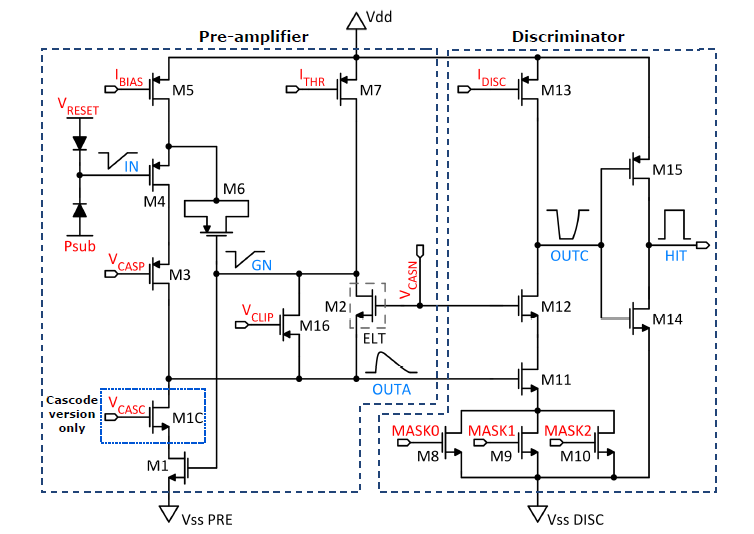
\includegraphics[scale=.75]{tj2-circuit}
\caption{Schematic of the improved front-end circuit and its variation (extra-cascode transistor) in TJ-Monopix2.}
\label{fig:tj2_circuit}
\end{figure}


In the last two AC-coupled flavors the same improvements have been implemented, but here the different coupling causes an important loss in the collected charge, as verified during the testing phase of TJ-Monopix1 (50\% losses), due at most to additional parasitic capacitances. Thus a lot of efforts have been made to improve this aspect, working on the coupling capacitor values. A signal loss of 41.5\% has been reached in TJ-Monopix2, which is a relevant enhancement with respect to its predecessor~\cite{Moustakas:2021gjr}.



% --------------------------------------------
%	5.2 THRESHOLD AND NOISE
%---------------------------------------------

\section{Threshold and noise} \label{thresh_noise}


The most probable value (MPV) of the signal released by a Minimum Ionizing Particle (MIP) in the thin MAPS sensitive thickness ($\approx$ \SI{30}{\micro m}) is only about 2250~$e^{-}$ (assuming \SI{75}{e^{-}/\micro m} \cite{wermes_book2020}). This small signal is collected by 2 or more pixels and could be further reduced after radiation damage due to trapping effects. 
In MAPS sensors it is then crucial to set the discriminator threshold to very low values in order to retain high detection efficiency, even after radiation damage.

The minimum value of the global threshold, compatible with a stable detector operation, depends on two important figures of merit: the noise and the threshold dispersion across the matrix. \\

\textbf{Noise and equivalent noise charge}. Electronic noise from the sensor diode and the pre-amplifier transistor (or other) devices results in time-varying voltage fluctuations at the pre-amplifier output. The Root Mean Square (RMS) of the voltage fluctuations is called noise output voltage.  
To quantify the noise of a readout channel the equivalent noise charge (ENC) is introduced, defined as the corresponding charge, in electrons, at the input of the channel that gives an output signal equal to the RMS noise output voltage.

\begin{equation}
ENC = \frac{noise \, output \, voltage \, (V)}{gain \, (V/e^{-})} 
\label{eq:ENC}
\end{equation}

\bigskip

\textbf{Operating threshold and threshold dispersion.} 
The global detection threshold has to be set to a value as low as possible in order to maximize the detection efficiency, but not too low in order to keep the noise hits at an acceptable level. Therefore the operating threshold value is ideally located between the noise peak around the baseline and the signal distribution. 
The dispersion of the threshold across the pixel matrix originates from the fabrication process variations and the mismatch of the integrated electronic components. These process related effects are responsible for dispersion of the quiescent voltage at the output of the pre-amplifier (baseline dispersion) and also for dispersion of the discriminator voltage offset, both contributing to the dispersion of the detection threshold. 

The threshold and its dispersion are also usually quantified reporting the corresponding charge, in electrons, at the input of the channel that gives an output signal corresponding to the threshold voltage and its dispersion:

\begin{align}
THR (e^{-}) & = \frac{voltage \, threshold \, (V)}{gain \, (V/e^{-})} \label{eq:th_gain} \\[2ex]
\sigma_{thr} (e^{-})    & = \frac{threshold \, dispersion \, (V)}{gain \, (V/e^{-})} 
\label{eq:disp_gain}
\end{align}

\medskip
The noise sets a lower bound to the threshold, but does not determine the stable operating threshold value which additionally depends on how the threshold varies with time and from pixel to pixel. The operating threshold lower limit is chosen to be at least approximately 5-6 times higher than the combined standard deviation of noise and threshold dispersion:

\begin{equation}
THR=(5-6) *\sqrt{ENC^{2} + \sigma_{thr}^{2}}
\end{equation}

\medskip
Therefore, apart from the global threshold, the possibility to fine tune the threshold locally per pixel is usually included in order to compensate these variations and is realized by digital to analog converters (DACs). The dispersion of the threshold after tuning is inversely proportional to the number of bits of the tuning DAC (TDAC):

\begin{equation}
\sigma_{thr,tuned} = \frac{\sigma_{thr}}{2^{n_{dac}}}
\end{equation}


\medskip
Since both the ENC (\autoref{eq:ENC}) and the threshold dispersion (\autoref{eq:disp_gain}) are inversely proportional to the gain, a lower global threshold could be achieved increasing the gain, through an optimized choice of chip registers.

To measure the threshold and noise of the whole matrix, the response of each pixel has been characterized by internal charge injection. \\


\subsection{Injection circuit} 
\label{sec:inj_circuit_subsection}

The hit injection circuit included in TJ-Monopix2, allows to produce artificial hits on each pixel through an injection capacitance \textbf{$C_{inj}$} connected at the collection electrode. The injected charge is proportional to the injection voltage pulse amplitude: $Q_{inj} = C_{inj} \cdot \Delta V_{inj}$. The injection pulse is set by two registers "\textbf{$V_{L}$}" and "\textbf{$V_{H}$}", with $\Delta V_{inj}$ = \textbf{$V_{H}-V_{L}$}, and the minimum injection step is given by the DAC resolution, with the Least Significant Bit (LSB) = \SI{7.03}{mV}. 

The injected signal is then often expressed in DAC units $Q_{inj}(DAC)$ and can be converted to electrons using the design value of the injection capacitance \textbf{$C_{inj}$} = \SI{230}{aF}, the same value for all FEs implemented.  
The nominal conversion factor $K$ from DAC to $e^{-}$ corresponds to the injected charge given by a voltage step of \SI{1}{DAC}: 

\begin{equation}
\normalsize
K = C_{inj} \cdot LSB = \frac{230 \, aF}{q_{{e}^{-}}} \cdot 7.03 \frac{mV}{DAC}= 1.4375 \frac{e^{-}}{mV} \cdot 7.03 \frac{mV}{DAC} \approx 10.1 \frac{e^{-}}{DAC}  
\label{eq:conversion_factor}
\end{equation}


An absolute calibration of the conversion factor $K$ (i.e. of the injection capacitance $C_{inj}$) has been also performed using radioactive sources, as explained in~\autoref{sec:source_ana}, obtaining results in agreement within 10\% from the design value. 

The conversion factor of~\autoref{eq:conversion_factor} has been used to convert the information of the injected charge from DAC unit to electrons unit, useful for further analysis.
\\
The response of each pixel to internal injection has been measured to extract their threshold and noise with the \textit{S-curve method} explained in the next section. 
The four flavors have been analyzed separately to be able to study their main differences concerning their performance and features. 


%--------------------------------------------------------------------
\subsection{S-Curve method} \label{sec:threshold_subsection}

The response of the pixels is measured injecting different amounts of charge into each pixel a given number of times and recording the amount of registered hits (i.e. the signal is above the discriminator threshold). For each value of the input signal we measure the occupancy, or hit probability, as the fraction of events where the pixel has registered a hit. This occupancy has the typical S-curve shape shown in~\autoref{fig:ex_scurve} as an example. 

As the injected signal passes the discriminator threshold the pixel starts to register some hits, finally reaching a plateau corresponding to the total number of injected events. This behaviour produces a step function smeared by the fluctuation on the input signal due to the noise.  
The threshold of the pixel corresponds to the injected signal  that gives 50\% occupancy, while the noise influences the slope of the S-curve.  

Assuming a gaussian noise distribution the S-curve can be fitted with the Cumulative Distribution Function (CDF):

\begin{equation}
 CDF(x,\mu,\sigma) = \frac{1}{2} \cdot \bigg(1 + \textit{erf}\bigg(\frac{x-\mu}{\sigma \sqrt{2}}\bigg)\bigg)
\label{eq:s-curve}
\end{equation}

where "\textit{erf}" is the Gauss error function, $x$ is the injected signal, $\mu$ and $\sigma$ are the threshold and the noise of the pixel, respectively.  \\

This method allows to measure the noise and the threshold of all pixels and also the threshold dispersion across an entire FE.

\begin{figure}
\centering
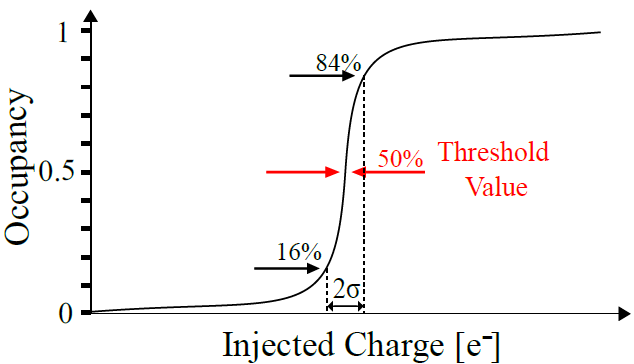
\includegraphics[scale=.7]{scurve_ex2}
\caption{An example of the S-Curve fitted by the CDF to evaluate threshold and noise.}
\label{fig:ex_scurve}
\end{figure}

In the following the results of this study for the four flavors of the matrix are reported. The injected signal was varied, with the corresponding voltage injection registers "VL,VH" , from 0 to \SI{140}{DAC}, corresponding to a charge of $\approx$ 1400~$e^{-}$, adopting the nominal conversion factor $K$ in~\autoref{eq:conversion_factor} .





\medskip
\begin{description}
\item \textbf{Normal FE}
\end{description}

The first flavor of the matrix is the \textbf{Normal FE}, which consists of 512 rows and 224 columns for a total of 114.688 pixels. The chip registers have been set with the same values used during the Test Beam at Desy (June 2022), which are different for the DC and AC-coupling cases. The most relevant among those responsible for the FE working point are reported in~\autoref{tab:tb_settings}, where the different biasing voltages used to power up the chip are also added. At the time of this first Test Beam campaign the front-end registers were still not  optimized to reach low threshold values. 

\begin{table}[h!]
\centering
\begin{tabular}{C{3.2cm}|C{3.7cm}|C{3.5cm}}
\hline
Registers & Normal/Cascode FE ($P_{SUB}$/$P_{WELL}$ = -3 V) & HV/HV-Cascode FE ($P_{SUB}$/$P_{WELL}$ = 0 V, HV = +5 V)\\[2ex]
\hline
\hline
$I_{THR}$ & 64 & 30\\[0.5ex]
\hline
$I_{BIAS}$ & 50 & 60\\
\hline
$V_{RESET}$ & 143 & 100\\
\hline
$I_{CASN}$ & 0 & 8\\
\hline
$I_{DB}$ & 100 & 100\\
\hline
$I_{TUNE}$ & 53 & 53\\
\hline
\hline
\end{tabular}
\caption{Settings of the main registers used for all flavors (W14R12 chip) during the Test Beam in Desy. The register meaning is explained in~\autoref{sec:currents}.}
\label{tab:tb_settings}
\end{table}


\begin{figure}[h!]
\centering
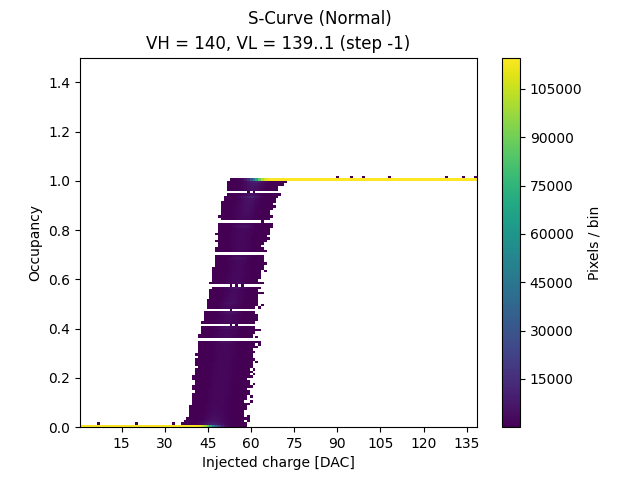
\includegraphics[scale=.5]{all_norm_thscan_140}
\caption{S-curves of all pixels of the Normal FE with a maximum injection pulse of \SI{140}{DAC}.}
\label{fig:norm_scurve_140}
\end{figure}


In~\autoref{fig:norm_scurve_140} the S-curves of the all Normal flavor pixels are plotted. The width of the figure is a first indication of the threshold dispersion across the whole flavor.
For each pixel the S-curve was fitted with the function in~\autoref{eq:s-curve} to extract their threshold and noise.  
The threshold and noise distributions measured for all pixels of the Normal FE sub-matrix are shown in~\autoref{fig:thdist_norm},  with their maps too. A fit with a gaussian distribution is used to extract the average threshold and noise values and their dispersion across the sub-matrix, and results are summarized in \autoref{tab:th_noise_all}.\\

\begin{figure}[h!]
\centering
\subfigure[Threshold distribution]
{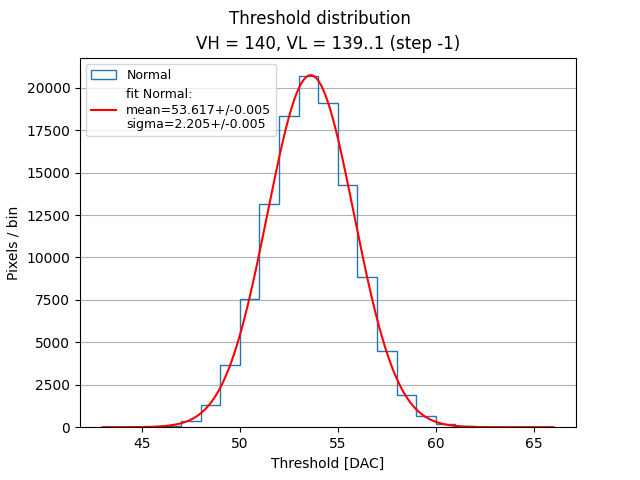
\includegraphics[scale=0.4]{all_norm_thdist_140}}\quad
\subfigure[Threshold map]
{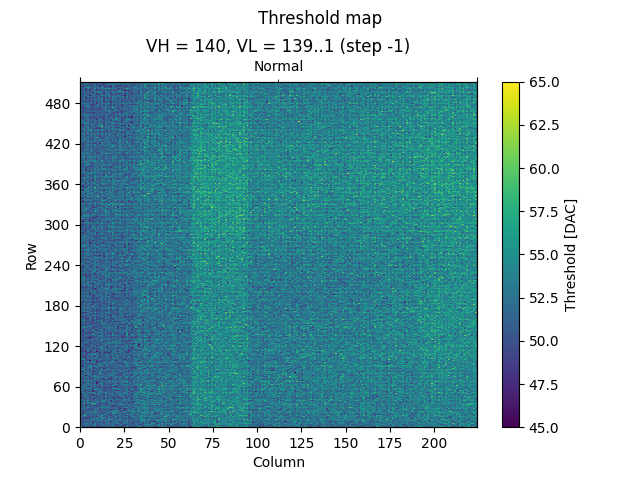
\includegraphics[scale=0.4]{threshold_map_norm_140_2}}\\
\subfigure[Noise distribution]
{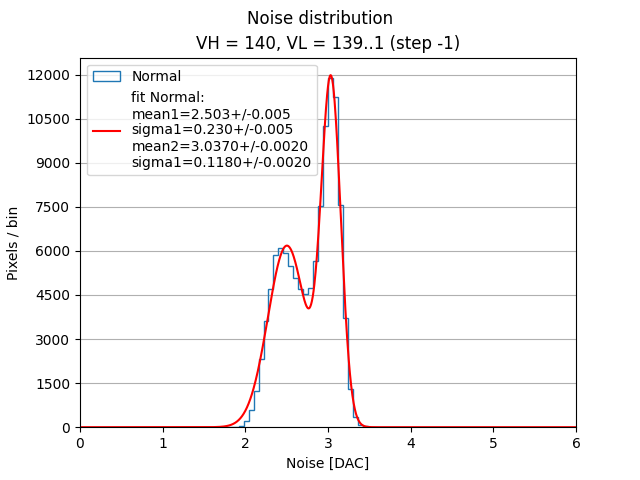
\includegraphics[scale=0.4]{Noise_hist_norm_140_fit2}}\quad
\subfigure[Noise map]
{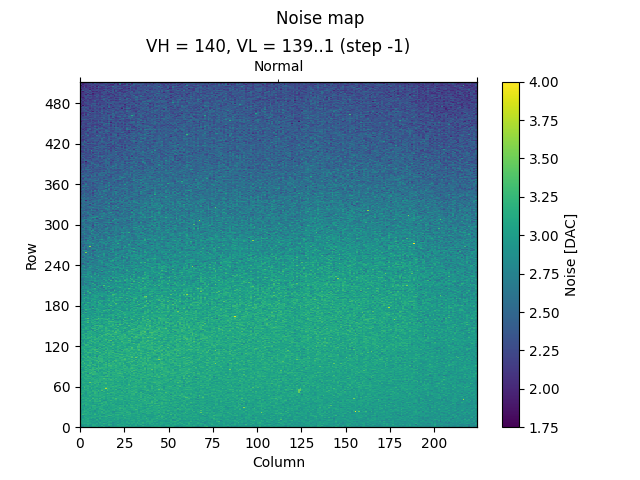
\includegraphics[scale=0.4]{Noise_map_norm_140_lim}}\\
\caption{Distributions and maps of threshold (first row) and noise (second row) in the entire Normal flavor.}
\label{fig:thdist_norm}
\end{figure}

The striped pattern visible in the threshold map, is due to the power distribution network.
In more detail, the matrix power pads are distributed along its left and right sides (\autoref{fig:tj2matrix}), therefore the voltage drop across the matrix analog power grid is compensated by using a local analog matrix supply, for groups of 32 columns \cite{Moustakas:2021gjr}, which determine this pattern.

The noise map shows a different behaviour in the upper part of the flavor, which has a smaller noise value on average, with respect to the lower part, where it results higher. We did not investigate further this behaviour in this phase of the characterization, although we believe the effect was eliminated by a change in the chip operating conditions.


\medskip
\begin{description}
\item \textbf{Cascode FE}
\end{description}

The \textbf{Cascode FE} is the second flavor and, like the previous one, it consists of 512 rows and 224 columns for a total of 114.688 pixels. For this flavor the same procedure of the Normal FE has been followed and the same registers' values (\autoref{tab:tb_settings}) have been used.
In~\autoref{fig:casc_scurve140} the S-curves of all pixels are shown.

\begin{figure}[h!]
\centering
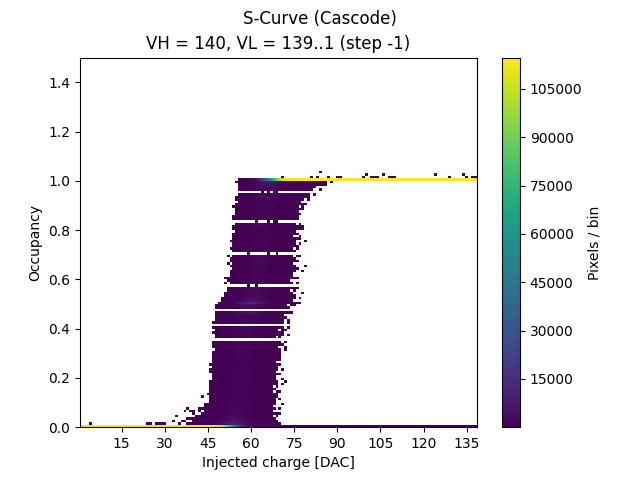
\includegraphics[scale=.5]{all_casc_thscan_140}
\caption{S-curves of all pixels in the Cascode flavor with a maximum injection pulse of \SI{140}{DAC}.}
\label{fig:casc_scurve140}
\end{figure}

The distributions of threshold and noise extracted with the fit to the S-curve, and their maps, are shown in~\autoref{fig:thdist_casc}. 
The striped pattern due to the power distribution network is less evident, and the noise map is more uniform, too. Results for Cascode FE flavor are also summarized in \autoref{tab:th_noise_all}.


\begin{figure}[h!]
\centering
\subfigure[Threshold distribution]
{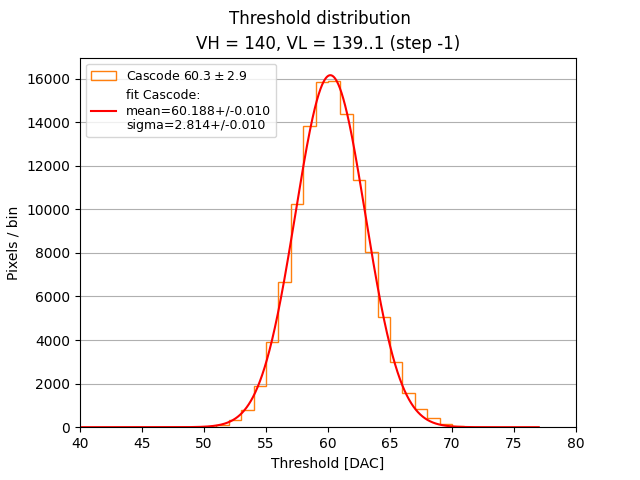
\includegraphics[scale=0.4]{all_casc_thdist_140}}\quad
\subfigure[Threshold map]
{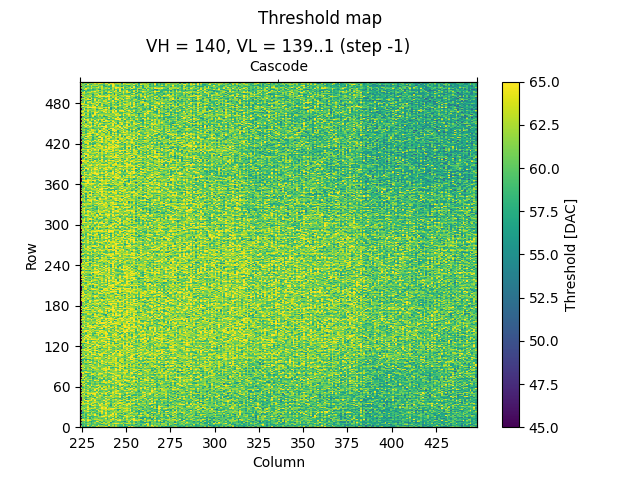
\includegraphics[scale=0.4]{threshold_map_casc_140_2}}\\
\subfigure[Noise distribution]
{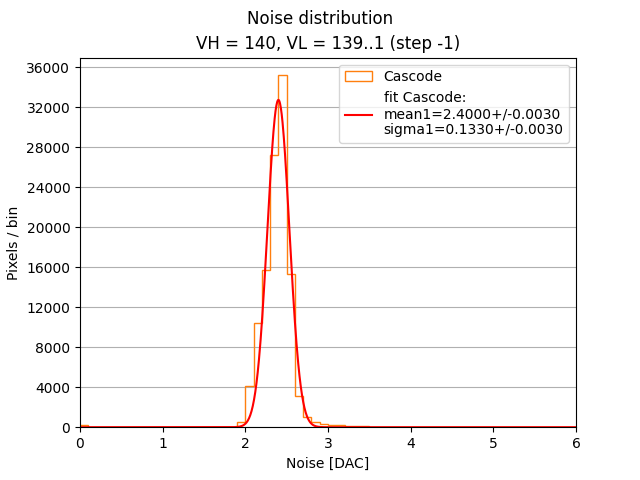
\includegraphics[scale=0.4]{Noise_hist_casc_140_fit2}}\quad
\subfigure[Noise map]
{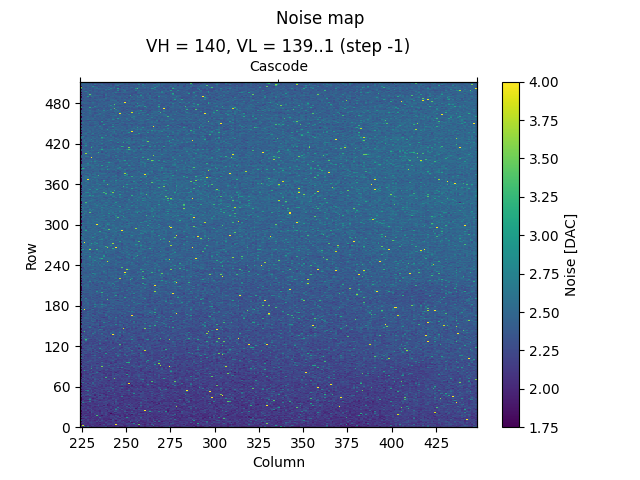
\includegraphics[scale=0.4]{Noise_map_casc_140_lim}}\\
\caption{Distributions and maps of threshold (first row) and noise (second row) in the entire Cascode flavor.}
\label{fig:thdist_casc}
\end{figure}


\medskip
\begin{description}
\item \textbf{HV-Cascode FE}
\end{description}

The third flavor is \textbf{HV-Cascode FE} and it is composed by 512 rows and 32 columns for a total number of pixel equal to 16384. Also for these last two flavors, the main chip registers are set with the same values tested and used during the Test Beam (but different from those used for the first two flavors). They are reported in the second column of~\autoref{tab:tb_settings}.

As we can see from the plot of all the S-curves in~\autoref{fig:hvc_scurve_140}, with this choice of registers there were a lot of "hot" pixels with occupancy > 1, but at this stage of measurements they were not masked.
These hot pixels with occupancy > 1, register more hits than the number of injected events. This behaviour seems to indicate that they are stimulated, not by the charge injection itself, but by some other input, active during the readout of the matrix, causing "cross-talk". The origin of the hot pixels and cross-talk was carefully investigated later (see~\autoref{sec:xtalk})
.

\begin{figure}[h!]
\centering
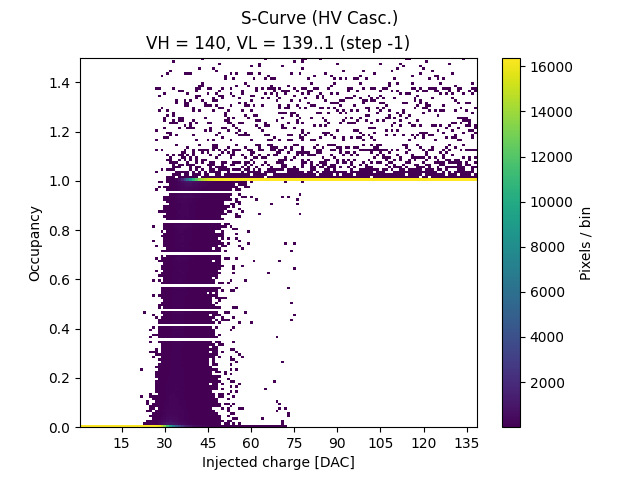
\includegraphics[scale=.5]{all_HVc_thscan_140}
\caption{S-curves of all pixels in HV Cascode flavor with a maximum injection pulse of \SI{140}{DAC}.}
\label{fig:hvc_scurve_140}
\end{figure}

In~\autoref{fig:thdist_hvc} the fits of the threshold and noise distributions are shown.

\begin{figure}[h!]
\centering
\subfigure[Threshold distribution]
{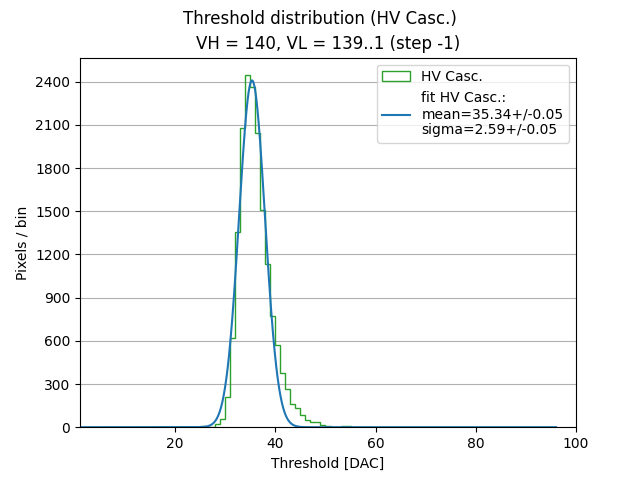
\includegraphics[scale=0.4]{all_HVc_thdist_140}}\quad
\subfigure[Noise distribution]
{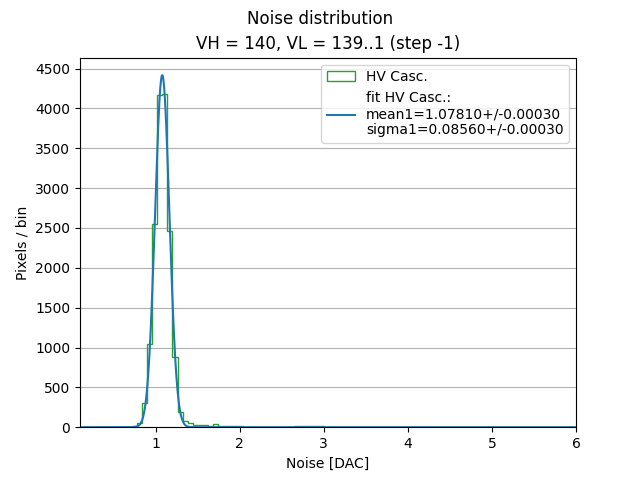
\includegraphics[scale=0.4]{Noise_hist_HV Casc._140_fit2}}\\
\caption{Distributions of threshold (a) and noise (b) in the entire HV Cascode flavor.}
\label{fig:thdist_hvc}
\end{figure}


\medskip
\begin{description}
\item \textbf{HV-Normal FE}
\label{sec:first_xtalk}
\end{description}

%\label{sec:first_xtalk}

The fourth and last flavor is the \textbf{HV-Normal FE} which has the same layout of the previous FE. The main registers have been set with the values reported in the second column of~\autoref{tab:tb_settings}.
The S-curves of all pixels in this flavor are shown in~\autoref{fig:hv_scurve_140} and we can notice some hot unmasked pixels, with occupancy > 1.
Moreover, the last 16 columns were not working and they returned a peak of threshold near the value 0, which is excluded from the threshold distribution plots.

Therefore in this part of the matrix, the real number of pixel studied was 8192, half of the total (visible in the maps in~\autoref{fig:HVs_maps}, where the last 16 columns are dark in color, corresponding to zero threshold and noise values).


\begin{figure}[h!]
\centering
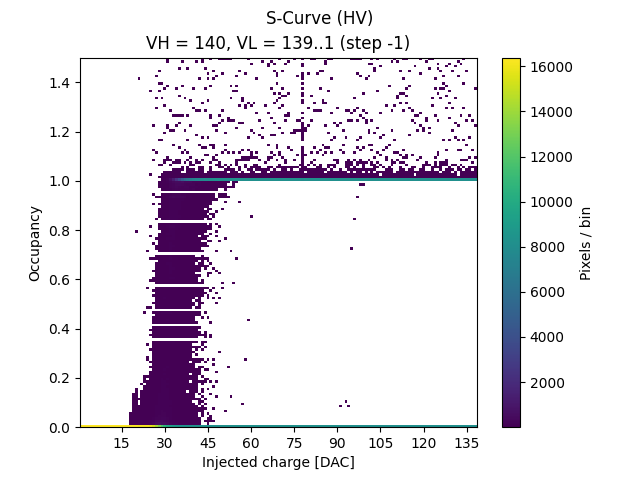
\includegraphics[scale=.4]{all_HV_thscan_140}
\caption{S-curves of all pixels in HV Normal FE with a maximum injection pulse of \SI{140}{DAC}.}
\label{fig:hv_scurve_140}
\end{figure}

In~\autoref{fig:thdist_hv} the fits of the threshold and noise distributions oh the HV-Normal, and in~\autoref{fig:HVs_maps} the threshold and noise maps of the whole HV flavors, are shown. 

\begin{figure}[h!]
\centering
\subfigure[Threshold distribution]
{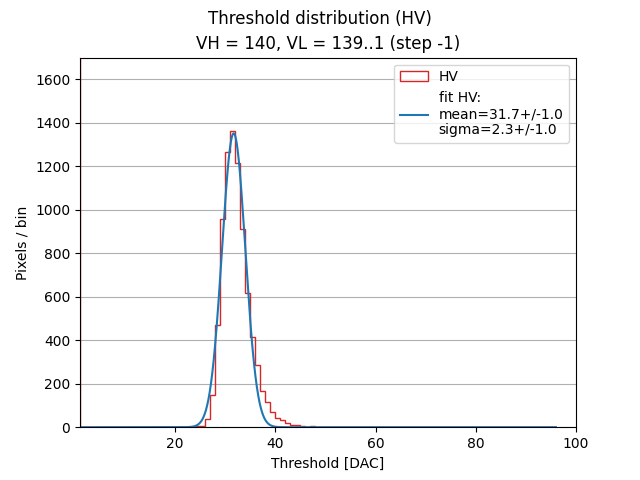
\includegraphics[scale=0.37]{all_HV_thdist_140}}\quad
\subfigure[Noise distribution]
{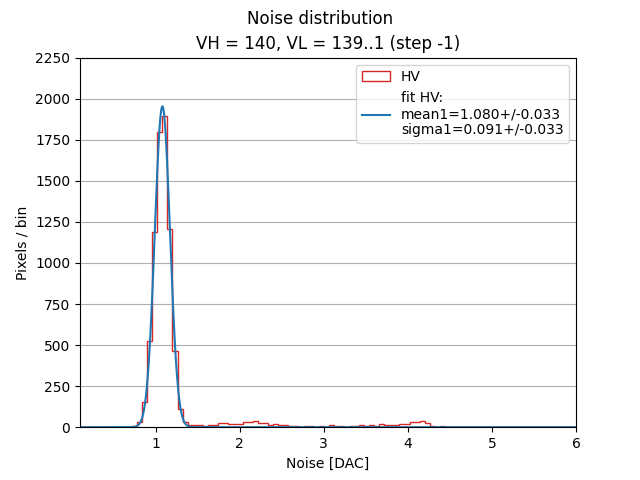
\includegraphics[scale=0.37]{Noise_hist_HV_140_fit2}}\\
\caption{Distributions of threshold (a) and noise (b) in the entire HV Normal flavor.}
\label{fig:thdist_hv}
\end{figure}

\begin{figure}[h!]
\centering
\subfigure[Threshold map]
{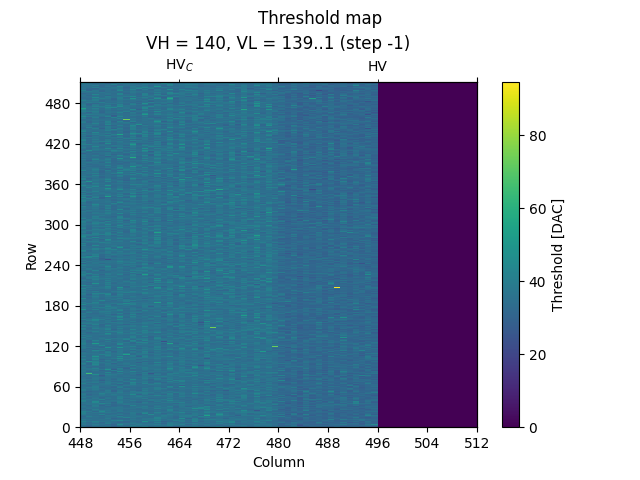
\includegraphics[scale=0.4]{threshold_map_All FEs_140}}\quad
\subfigure[Noise map]
{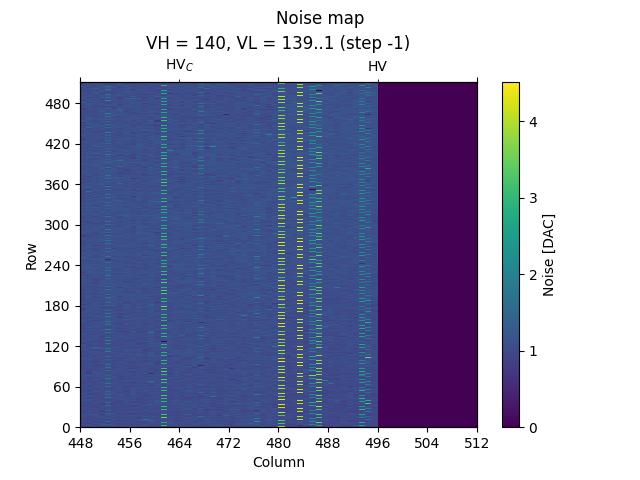
\includegraphics[scale=0.4]{Noise_map_HV_1402}}\\
\caption{Threshold (a) and noise (b) maps in HV Cascode (left 32 columns) and HV Normal FE (right 32 columns).}
\label{fig:HVs_maps}
\end{figure}

As we will see in the following (\autoref{sec:xtalk}), the atypical S-curves with many hot pixels in the HV flavors, have been the first hint of the cross-talk problem, tied to a global lower threshold in these sectors, compared with the first two thresholds measured in the Normal and Cascode sector (with the Test Beam settings). 

\newpage
\subsection{Threshold, noise ad threshold dispersion results (Test Beam settings)}\label{sec:th_summary}

In~\autoref{tab:th_noise_all} a summary of the results for threshold, noise and threshold dispersion of all the FE is reported, both in DAC and in $e^{-}$ unit, using the nominal conversion factor $K$ in~\autoref{eq:conversion_factor}.

\begin{table}[h!]
\centering
\begin{tabular}{C{2cm}|C{1.6cm}|C{1.6cm}|C{1.8cm}|C{1.6cm}|C{1.5cm}|C{1.5cm}}
\hline
FE & Threshold [DAC] & Threshold [$e^{-}$] & Threshold dispersion [DAC] & Threshold dispersion [$e^{-}$] & Noise [DAC] & Noise [$e^{-}$]\\
\hline
\hline
Normal  & 53.6 & 541.6  & 2.2 & 22.3 & \shortstack{2.5 \\ 3.0} & \shortstack{25.3 \\ 30.7}\\
\hline
Cascode & 60.2 & 607.9 & 2.8 & 28.4 & 2.4 & 24.2\\
\hline
HV - Cascode & 35.3 & 356.9 & 2.6 & 26.2 & 1.1 & 10.9\\
\hline
HV & 31.7 & 320.0 & 2.3 & 23.0 & 1.1 & 10.9\\
\hline
\hline
Target (\autoref{tab:tj2_spec}) & & $\approx$ 100 & & $\le$10 & & $\le$ 8 \\
\hline
\end{tabular}
\caption{Summary table of threshold, threshold dispersion and noise values for all flavors of the W14R12 chip. The conversion from DAC to $e^{-}$ unit has been done using the nominal conversion factor K~=~\SI{10.1}{e^{-}/DAC}.}
\label{tab:th_noise_all}
\end{table}

The measured values are much higher than expected under convenient working conditions (optimized values shown in~\autoref{tab:tj2_spec}). However, as we have pointed out in the previous, we carried out the characterization of the matrix response adopting the TB register settings, to obtain results essential for the TB data reconstruction, and not to work in optimized conditions.

In~\autoref{sec:low_thr} we will show some test results, trying to operate the chip at low threshold.


%--------------------------------------------------------------------

%--------------------------------------------------------------------
\section{TOT calibration with internal injection}


The analog information on the signal height is provided by the Time Over Threshold (\autoref{fig:ToT}) digitized with a \SI{25}{ns} clock (the Bunch Crossing ID (BCID) clock-frequency is \SI{40}{MHz}). 

\begin{figure}[h!]
\centering
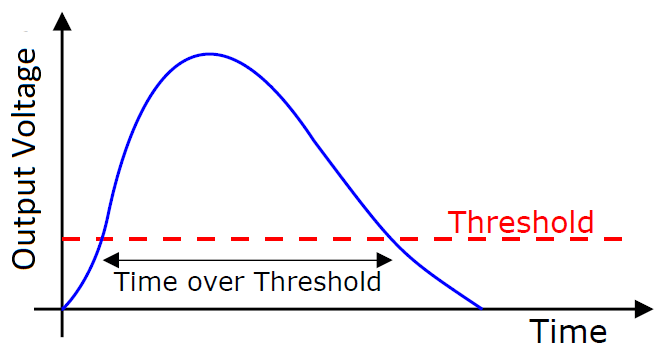
\includegraphics[scale=.7]{TOT1}
\caption{Time Over Threshold (TOT) method to encode the voltage analog information.}
\label{fig:ToT}
\end{figure}

The choice to use a simple diode (instead of a PMOS transistor) as reset input baseline element, increases the tolerance to Total Ionizing Dose (TID) radiation, but it also implies a difficult to model relationship between the injected charge and the TOT. For this reason, one of the goal of this analysis was to measure the calibration curve TOT vs $Q_{inj}$ via the internal injection. The fit to the calibration curve allows to find the conversion function needed to reconstruct the signal amplitude, measuring its TOT. It also allows an absolute calibration of the injection capacitance, done comparing the results of the TOT response from the radioactive source with known released signal, with the response to the same signal through the injection circuit.

In carrying out the measurements mentioned above, we started to notice some issues with the injection circuit, which showed some saturation in the voltage pulse at high values of the registers. Due to this issue, the TOT response to internal injection could only be measured up to 170 DAC ($\approx$ 1700~$e^{-}$). This was enough for the absolute calibration using the \ch{^{55}Fe} \SI{5.9}{KeV} emission line ($\approx$ 1616~$e^{-}$) as explained below (\autoref{sec:source_ana}).\\
A method has been therefore devised to obtain reliable values of threshold and TOT up to a value of 170 DAC of effective charge injected.

The calibration function adopted to describe the $Q_{inj}$-TOT relationship was then used to extrapolate TOT values in the region of high charge (above 170 DAC, $\approx$ 1700 $e^{-}$) not accessible with the injection circuit, to compare with the emission peaks of other radioactive sources and explore a larger range (\autoref{sec:check}).


%--------------------------------------------------------------------
\subsection{TOT curves and fit} \label{sec:tot_fit}

The characterization of the function that reproduces the $Q_{inj}$-TOT relationship is crucial to convert the TOT information returned by the chip to the actual charge collected. These measurements have also been taken using the Test Beam register settings (\autoref{tab:tb_settings}), thus allowing the reconstruction of TB data.

Given the shape of the TOT distribution depending on the injected charge shown in Figure~\autoref{fig:tot_shape}, the empirical function chosen to describe the calibration curve is:

\begin{equation}
y(x) = a\cdot x +b -\frac{c}{x-t}
\label{eq:fit_function}
\end{equation}

with \textit{a}, \textit{b}, \textit{c} and \textit{t} free parameters and where \textit{y} represents the TOT corresponding to the value of collected charge, expressed by \textit{x}.

For calibration purposes it would be necessary to fit the TOT distribution of each pixel, but at this stage, we need to characterize the overall response of each FE. Therefore, we have computed the average value of the TOT distribution of all pixels in each flavor. The several steps done to improve the results are explained in the following, considering the TOT curve of the Normal FE as example.\\

\begin{figure}[h!]
\centering
\subfigure[\label{fig:tot_shape} TOT curve]
{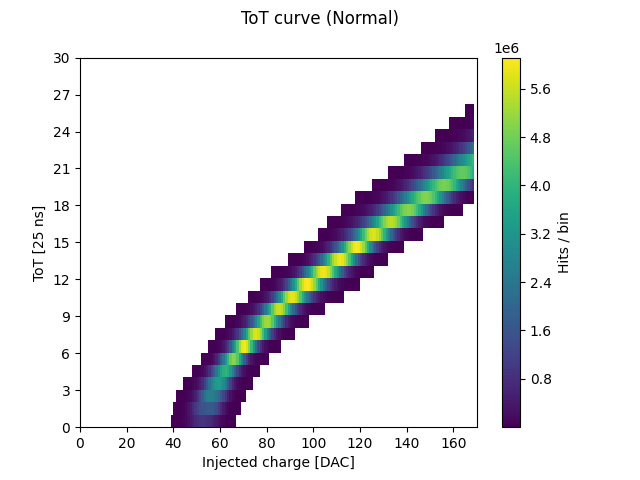
\includegraphics[scale=0.5]{ToT_vs_Q_norm}}\\
\subfigure[\label{fig:tot_mean}Weighted average on TOT for each charge bin.]
{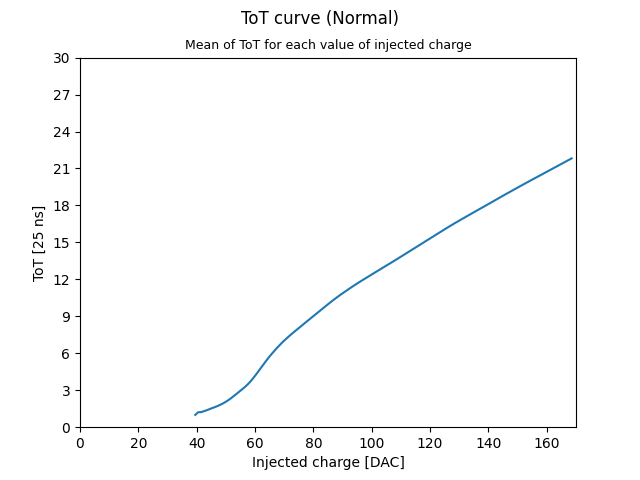
\includegraphics[scale=0.42]{mean_on_tot_norm2}}\quad
\subfigure[\label{fig:charge_mean}Weighted average on charge for each TOT bin.]
{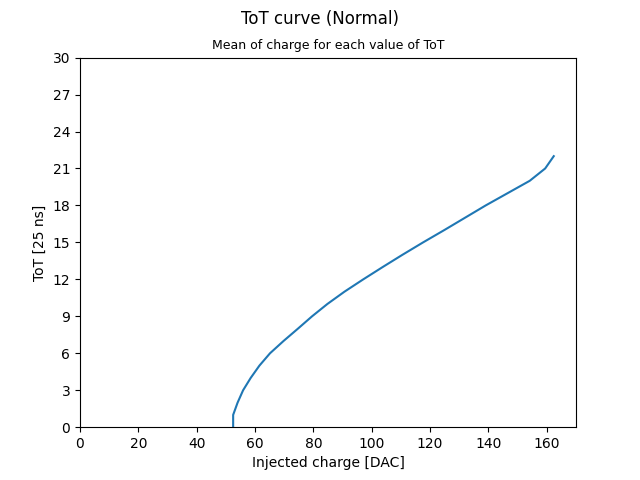
\includegraphics[scale=0.42]{mean_on_charge_norm2}}\\
\subfigure[\label{fig:fit_tot}Fit of the weighted average TOT values for each charge bin, using eq.~\ref{eq:fit_function}, all parameters free.]
{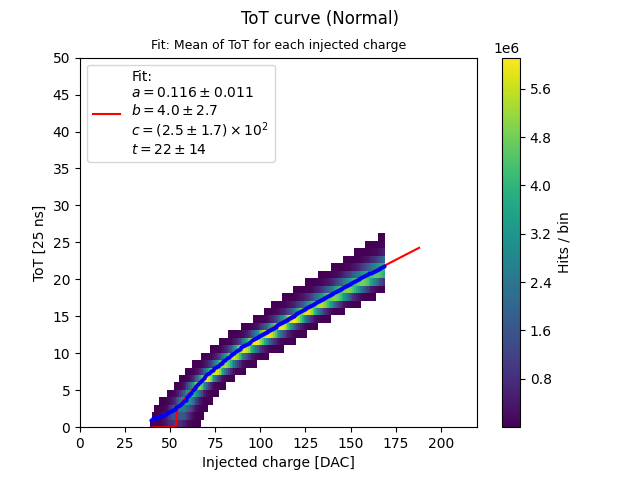
\includegraphics[scale=0.43]{totfit_meantot_nocos_norm2}}\quad
\subfigure[\label{fig:fit_charge}Fit of the weighted average charge values for each TOT bin, using eq.~\ref{eq:fit_function}, all parameters free.]
{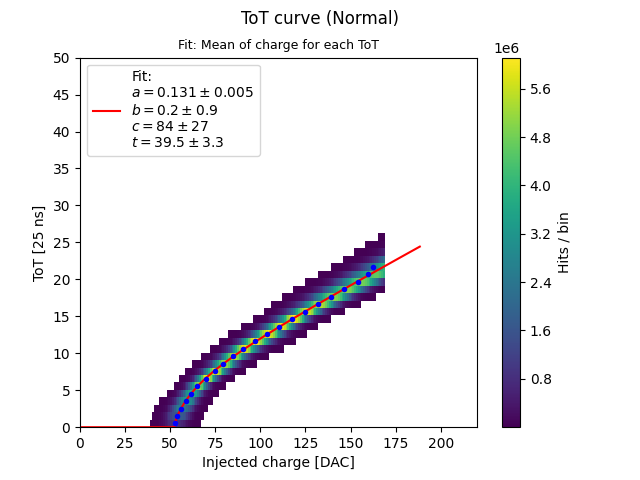
\includegraphics[scale=0.43]{tot_meancharge_nocos_norm2}}
\caption{Characterization of the calibration function for the Normal FE.}
\end{figure}


%FIRST STEP
At first the weighted average of the TOT values for each injected charge bin was calculated and the result is displayed in Figure~\autoref{fig:tot_mean}.
As we can see, this method does not reproduce the TOT distribution shape at low values very well, since due to the threshold dispersion on the flavour, there are low TOT values corresponding to injected charges lower than the global threshold of the FE, estimated in the previous (\autoref{tab:th_noise_all}). For this reason the weighted average on TOT near the threshold does not go to zero as expected. 

%SECOND 
To improve the reproduction of the TOT distribution shape at low values, we made the weighted average of the charge for each TOT bin. The result is reported in Figure~\autoref{fig:charge_mean}, and the shape obtained is much more in agreement with the distribution in Figure~\autoref{fig:tot_shape}. Therefore we tried to fit both dataset with the function in~\autoref{eq:fit_function}, leaving all parameters free. In Figure~\autoref{fig:fit_tot} and in Figure~\autoref{fig:fit_charge} are reported the fit of the weighted average values on TOT and on charge, respectively. To compare the fit results, we calculated the relative error for each parameter, reported in~\autoref{tab:fit_table}. The first two columns, corresponding to the results obtained in these two first steps, show that this adjustment has also improved the uncertainties on the parameters, except for \textit{b}, whose value is of the same order of its uncertainty.

Although the averaged values on the charge returned smaller, but not yet acceptable errors, we tried to repeat the fit on the weighted average TOT values, cutting the low TOT points between 0 and 5 TOT unit (with a BCID clock frequency of \SI{40}{MHz}, one TOT unit corresponds to \SI{25}{ns}).

The parameter values obtained are shown in figure~\autoref{fig:tot_mean2}, and their relative uncertainties in the third column of~\autoref{tab:fit_table}. As we can see, fitting the cut data returned smaller uncertainties on the parameters. 

\begin{figure}[h!]
\centering
\subfigure[\label{fig:tot_mean2}Fit of the weighted average TOT values ($\le$~5) for each charge bin, using eq.~\ref{eq:fit_function}, all parameters free.]
{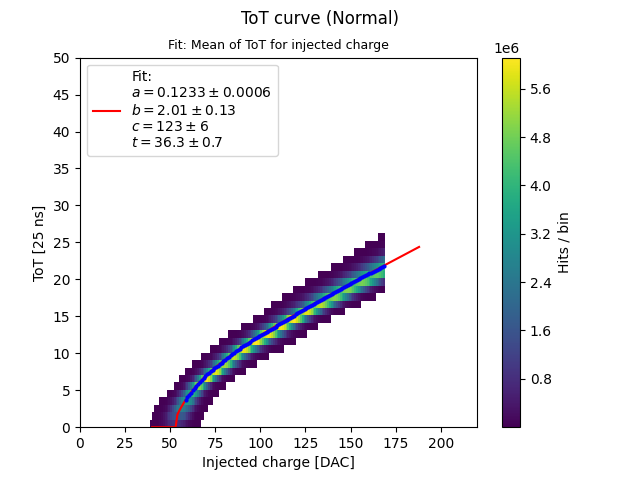
\includegraphics[scale=0.44]{totfit_meantot_nocos_norm_cut}}\quad
\subfigure[\label{fig:totfit_third}Fit of the weighted average TOT values ($\le$~5) for each charge bin, using eq.~\ref{eq:fit_function2}, with \textit{a}, \textit{b} and \textit{t} left free and \textit{c} computed using~\autoref{eq:c_param}.]
{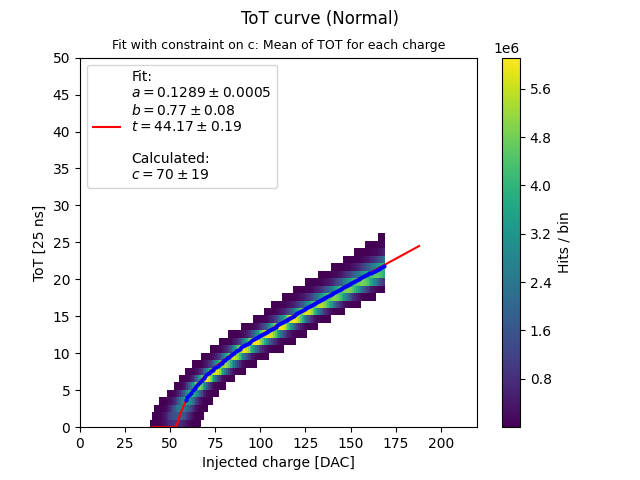
\includegraphics[scale=0.44]{totfit_meantot_ccos_norm2}}\\
\caption{Characterization of the calibration function for the Normal FE.}
\end{figure}


%THIRD
To further enhance the characterization of the calibration function, we have exploited the information on the global threshold of the FEs (\autoref{tab:th_noise_all}).
The TOT distribution starts to grow near the threshold, then one of the four free parameters could be computed as a function of its value because, from~\autoref{eq:fit_function}, knowing that y($x_{th}$) must be equal to 0 (that is the TOT value at the threshold), it can be imposed:

\begin{equation}
0 = a\cdot x_{th} + b - \frac{c}{x_{th}-t}  \hspace{.4cm}	\Rightarrow  \hspace{.4cm}	c = x_{th}^{2}\cdot a + x_{th}\cdot (b-a\cdot t) - t\cdot b
\label{eq:c_param}
\end{equation}

\medskip
So the function to fit the TOT curve becomes:
\begin{equation}
y(x) = a\cdot x +b -\frac{x_{th}^{2}\cdot a + x_{th}\cdot (b-a\cdot t) - t\cdot b}{x-t}
\label{eq:fit_function2}
\end{equation}

with a number of parameters to fit reduced from four to three (\textit{a}, \textit{b} and \textit{t}).

In~\autoref{fig:totfit_third} the results obtained for the Normal FE. The parameter \textit{c} was calculated using the~\autoref{eq:c_param} and its uncertainty was evaluated using the error propagation formula, including the threshold dispersion as uncertainty of the threshold value.\\

The relative uncertainties on parameters are reported in the fourth column of~\autoref{tab:fit_table}. The uncertainties on parameters \textit{a} and \textit{t} are reduced, but those on \textit{b} and \textit{c} are increased (in case of \textit{c}, due mostly to the threshold dispersion in its error propagation formula).


%TABLE COMPARISON FIT
\begin{table}[h!]
\centering
\begin{tabular}{C{1.1cm}|c|c|c|c}
 &  \shortstack{Weighted TOT\\ fit using eq.~\ref{eq:fit_function}\\ a, b, c, t free} &  \shortstack{Weighted charge \\ fit using eq.~\ref{eq:fit_function} \\ a, b, c, t free} &  \shortstack{Weighted TOT \\ (cutting TOT~<~5)\\ fit using eq.~\ref{eq:fit_function}\\ a, b, c, t free} & \shortstack{Weighted TOT \\ (cutting TOT~<~5)\\ fit using eq.~\ref{eq:fit_function2}\\ a, b, t free \\ c computed (eq.~\ref{eq:c_param})} \\[.5ex]
\hline
\hline \\[-2.5ex]
$\Delta$a/a & 9.6\% & 3.5\% & 0.5\% & 0.4\% \\ [0.5ex]
\hline
$\Delta$b/b & 67.5\% & 109.2\% & 6.3\% & 10.8\% \\[0.5ex]
\hline
$\Delta$c/c & 67.3\% & 38.3\% & 4.6\% & 27.7\% \\[0.5ex]
\hline
$\Delta$t/t & 60.6\% & 8.1\% & 2.0\% & 0.4\% \\[0.5ex]
\hline
\hline
\end{tabular}
\caption{Relative uncertainties of parameters obtained from the several fits of TOT curve for the Normal FE.}
\label{tab:fit_table}
\end{table}

There is a strong correlation between the four parameters, therefore improving the result on one of them, could worsen the result on another, as we can see from ~\autoref{tab:fit_table}. We have observed the same trend (with different percentages) of the uncertainties also for the other FEs. \\


\subsection{Comparison}

To evaluate which of the fit results could best reproduce the TOT-$Q_{inj}$ relationship, we inverted the empirical calibration function (\autoref{eq:fit_function}) to obtain the value of the charge (\textit{x}) as a function of the TOT, \textit{a}, \textit{b}, \textit{c}, and \textit{t}:

\begin{equation}
x(y) = \bigg(\frac{t}{2} - \frac{b}{2a} + \frac{y}{2a}\bigg) \pm \sqrt{\bigg(\frac{t}{2} + \frac{b}{2a} - \frac{y}{2a}\bigg)^{2} + \frac{c}{a}}
\end{equation}

Knowing that for a zero TOT value (y), we should obtain the value of the threshold ($x_{th}$), we computed the uncertainty on the expression below, using the error propagation formula:

\begin{equation}
x(0) = x_{th} = \bigg(\frac{t}{2} - \frac{b}{2a}\bigg) \pm \sqrt{\bigg(\frac{t}{2} + \frac{b}{2a}\bigg)^{2} + \frac{c}{a}}
\label{eq:xth_merit}
\end{equation}

Between the two possible solutions we took the one with the "+", which returns the higher value and represents our threshold. The other solution instead represents nothing of our data, so it is discarded.

Then we compared this result with the threshold dispersion extracted from the threshold distribution fit (\autoref{tab:th_noise_all}). \autoref{tab:xth} shows the comparison: in the first row the threshold value and its dispersion for each FE, in the second row the same quantities estimated as described in the previous, using the parameter values (\textit{a}, \textit{b}, \textit{c} and \textit{t}) obtained by the fit method summarized in the third column of~\autoref{tab:fit_table}, while in the third row using the fit method summarized in the fourth column of the same table.

%TABLE DISPERSION
\begin{table}[h!]
\centering
\begin{tabular}{c|c|c|c|c}
 & \textbf{Normal} & \textbf{Cascode} & \textbf{HV Cascode} & \textbf{HV} \\[.5ex]
\hline
\hline \\[-2.5ex]
\shortstack{\textit{$x_{th}\pm\Delta x_{th}$} [DAC] \\ from the threshold distribution fit} & 53.6$\pm$2.2 & 60.2$\pm$2.8 & 35.3$\pm$2.6 & 31.7$\pm$2.3 \\ [0.5ex]
\hline
\shortstack{\textit{$x_{th}\pm\Delta x_{th}$} [DAC] \\ from $x_{th}$(a,b,c,t) in eq.~\ref{eq:xth_merit}\\ using a,b,c,t from 3° column of~\autoref{tab:fit_table}} & 51.1$\pm$0.2 & 64.2$\pm$0.4 & 35.1$\pm$2.7 & 31.5$\pm$2.6 \\[0.5ex]
\hline
\hline
\shortstack{\textit{$x_{th}\pm\Delta x_{th}$} [DAC] \\ from $x_{th}$(a,b,c,t) in eq.~\ref{eq:xth_merit} \\ using a,b,c,t from 4° column of~\autoref{tab:fit_table}} & 53.4$\pm$2.2 & 60.8$\pm$2.7 & 35.1$\pm$2.7 & 31.5$\pm$2.4 \\[0.5ex]
\hline
\hline
\end{tabular}
\caption{In the first row the the threshold value and its dispersion for each FE (\autoref{tab:th_noise_all}); in the second row the same quantities estimated by eq.~\ref{eq:xth_merit} and their uncertainties, using parameter values obtained from the third fit method (third column in~\autoref{tab:fit_table}); in the third row same procedure but using parameter values from the fourth fit method (fourth column in~\autoref{tab:fit_table}).}
\label{tab:xth}
\end{table}

The agreement with data in the first row, is obtained with parameter values extracted from the fourth fit method, even though the parameter uncertainties (\autoref{tab:fit_table}) are higher compared to the parameter results obtained without condition on \textit{c}. It is worth to mention that in the third fit method, parameters are estimated cutting data near the threshold, which is what we want to return with this procedure, therefore we do not expected the results to be in agreement.\\

% TOT at Fe peak
Finally, we extracted the expected TOT value corresponding to the charge released from the \SI{5.9}{KeV} emission line of \ch{^{55}Fe} source, to compare it with the peak measured during the acquisitions with the source, shown in~\autoref{fig:fe_all}. We computed the TOT value using~\autoref{eq:fit_function} for parameter values obtained without condition on \textit{c} parameter, and~\autoref{eq:fit_function2} for parameters obtained with the last fit method. The results are reported in~\autoref{tab:tot_fe}, together with the measured peak values. To calculate the expected charge in DAC corresponding to the charge released from the source ($\approx$ 1616~$e^{-}$) we used the nominal conversion factor $K$=\SI{10.1}{e^{-}/DAC} (\autoref{eq:conversion_factor}), as following:

\begin{equation}
Q_{exp}(DAC) = \frac{N_{e^{-}}}{K} = \frac{1616 \, e^{-}}{10.1 \, e^{-}/DAC} = 160 \, DAC    
\end{equation}

%TABLE TOT
\begin{table}[h!]
\centering
\begin{tabular}{c|c|c|c|c}
 & \textbf{Normal} & \textbf{Cascode} & \textbf{HV Cascode} & \textbf{HV} \\[.5ex]
\hline
\hline \\[-2.5ex]
\shortstack{TOT(160 DAC)$\pm\Delta$TOT [TOT unit] \\ from source acquisition} & 23.4$\pm$1.4 & 21.8$\pm$1.3 & 35.3$\pm$2.6 & 31.7$\pm$2.3 \\ [0.5ex]
\hline
\shortstack{TOT(160 DAC)$\pm\Delta$TOT [TOT unit] \\ from y(x,a,b,c,t) in eq.~\ref{eq:fit_function}\\ using a,b,c,t from 3° column of~\autoref{tab:fit_table}} & 20.8$\pm$1.4 & 19.4$\pm$1.3 & 35.1$\pm$2.7 & 31.5$\pm$2.6 \\[0.5ex]
\hline
\hline
\shortstack{TOT(160 DAC)$\pm\Delta$TOT [TOT unit] \\ from y(x,a,b,c,t) in eq.~\ref{eq:fit_function2}\\ using a,b,t from 4° column of~\autoref{tab:fit_table}} & 20.8$\pm$2.7 & 19.4$\pm$3.1 & 35.1$\pm$2.7 & 31.5$\pm$2.4 \\[0.5ex]
\hline
\hline
\end{tabular}
\caption{In the first row the the source peak value of \ch{^{55}Fe} and its dispersion for each FE (\autoref{fig:fe_all}); in the second row the same quantities estimated by~\autoref{eq:fit_function} and their uncertainties, using parameter values obtained from the third fit method (third column in~\autoref{tab:fit_table}); in the third row same procedure but using parameter values from the fourth fit method (fourth column in~\autoref{tab:fit_table}).}
\label{tab:tot_fe}
\end{table}

Although the results obtained from the fourth fit method return threshold and dispersion values more compatible with those measured via internal charge injection (\autoref{tab:xth}), the estimate of the TOT value corresponding to the iron emission peak and its dispersion, seem to be slightly more similar with the measured ones, using the parameters obtained from the third fit method. Moreover in this case, the relative uncertainties of the parameters are smaller. So in the following, we decided to fit the TOT curve with~\autoref{eq:fit_function} leaving all parameters free. In~\autoref{fig:totfit_cut} the fit results for all FEs are shown.


\begin{figure}[h!]
\centering
\subfigure[\textbf{Normal}]
{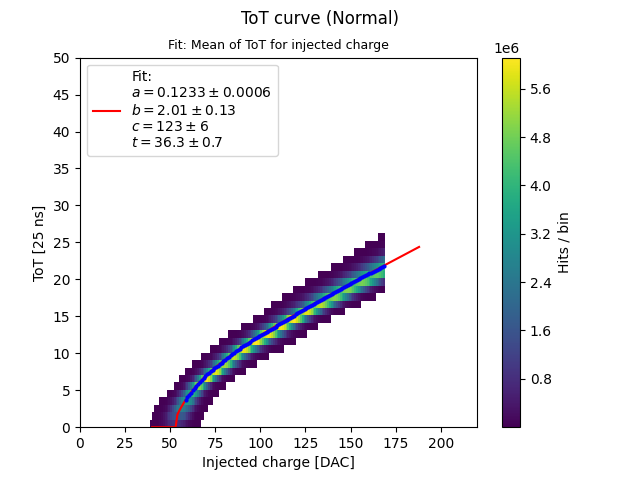
\includegraphics[scale=0.44]{totfit_meantot_nocos_norm_cut}}\quad
\subfigure[\textbf{Cascode}]
{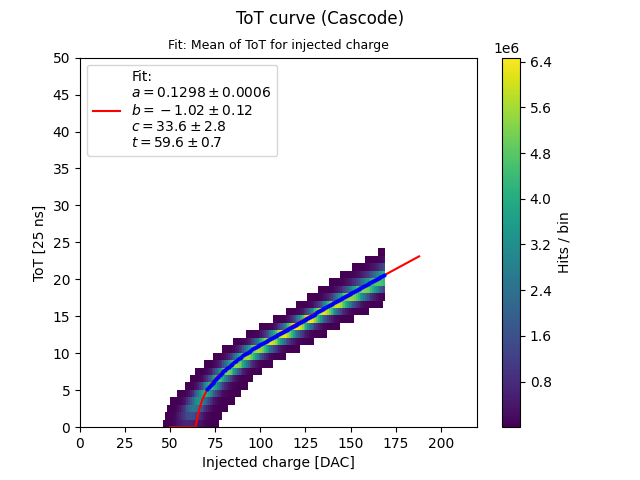
\includegraphics[scale=0.44]{totfit_meantot_nocos_casc_cut}}\\
\subfigure[\textbf{HV Cascode}]
{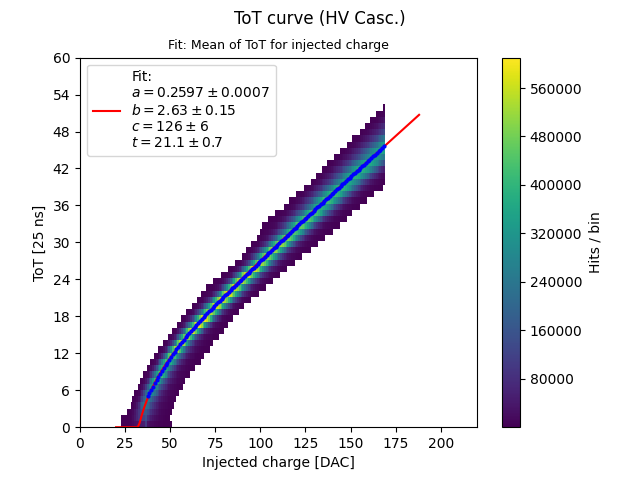
\includegraphics[scale=0.44]{totfit_meantot_nocos_HV Casc.cut}}\quad
\subfigure[\textbf{HV}]
{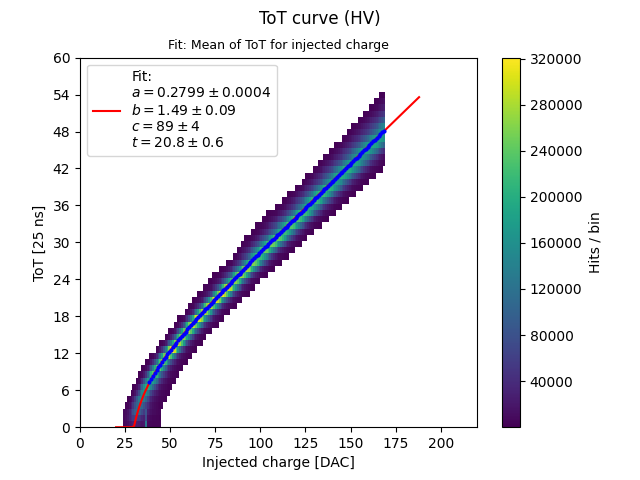
\includegraphics[scale=0.44]{totfit_meantot_nocos_HVcut}}\\
\caption{Fit of the weighted average TOT values ($\le$~5) for each charge bin, using~\autoref{eq:fit_function} to extract the values of \textit{a}, \textit{b}, \textit{c} and \textit{t}. The results for all FEs are shown.}
\label{fig:totfit_cut}
\end{figure}




\newpage
%--------------------------------------------------------------------
\section{Response to radioactive source and absolute calibration} \label{sec:source_ana}

%06/10/2022 LOGBOOK

After the characterization by the internal injection, we measured the response of the matrix to three different X-rays radioactive sources: \ch{^{55}Fe}, \ch{^{241}Am}, \ch{^{109}Cd}, with emission lines from 6 to \SI{60}{KeV}, corresponding approximately to a range between 1600 and 16000 $e^{-}$ signal charge released in the silicon, as shown in \autoref{tab:radio_sources}.

In this way we could perform the absolute calibration of the matrix response and extend the study of the TOT spectrum above the limit imposed by the saturation of the internal injection circuit ($\approx$ 1700 $e^{-}$). This is also useful to verify the goodness of the calibration curve characterization at higher signal, that could be deposited by a MIP due to the long tail of the Landau distribution, which describes the fluctuations of the energy released by a charged particle traversing a medium. 

The absolute calibration of the matrix consists in characterizing the response of each pixel to a known signal, like the emission peaks of radioactive sources, and then comparing the results with the response from the internal injection to the same amount of signal, as explained in \autoref{sec:inj_cap_calib}. 

The absolute calibration of the conversion factor of~\autoref{eq:conversion_factor}, equivalent to measuring the injection capacitance $C_{inj}$,  is performed with the \SI{5.9}{KeV} peak of the \ch{^{55}Fe} source ($\approx$ 1616 $e^{-}$), that is still in the range explored with the injection circuit. The other radioactive sources, with high energies, allowed to extend the TOT comparison at higher values with respect to the limit imposed by the saturation of the internal injection circuit. In~\autoref{tab:radio_sources} the energies of the $\gamma$ emitted by the sources used are shown.\\
%it is possible to convert
Considering that the average energy necessary to produce an electron/hole pair in silicon is \SI{3.65}{eV}, the peak energies expressed in KeV could be converted in a mean value of electrons released, using the~\autoref{eq:energy_electron_conv}. The equivalent emission lines in electrons unit, which will be useful later, are reported in the second column of ~\autoref{tab:radio_sources}

\begin{equation}
N_{e^{-}} = \frac{E \, [eV]}{3.65 [\frac{eV}{e/h \, pair}]}
\label{eq:energy_electron_conv}
\end{equation}


\begin{table}[h!]
\centering
\begin{tabular}{C{3cm}|C{2.8cm}|C{2.8cm}}
\hline
Source & Energy $\gamma$ [KeV] & Equivalent charge [$e^{-}$]\\[2ex]
\hline
\hline
\ch{^{55}Fe} & 5.9 & 1616\\[0.5ex]
\hline
\ch{^{241}Am} & 13.9 & 3808\\[0.5ex]
\hline
\ch{^{241}Am} & 17.7 & 4849\\[0.5ex]
\hline
\ch{^{241}Am} & 20.7 & 5671\\[0.5ex]
\hline
\ch{^{109}Cd} & 22 & 6027\\[0.5ex]
\hline
\ch{^{241}Am} & 26.4 & 7233\\[0.5ex]
\hline
\ch{^{241}Am} & 59.7 & 16356\\
\hline
\hline
\end{tabular}
\caption{Emission lines of \ch{^{55}Fe}, \ch{^{241}Am}, \ch{^{109}Cd} sources.}
\label{tab:radio_sources}
\end{table}


Now we can go through the results obtained from three different sources: \ch{^{55}Fe}, \ch{^{241}Am} and \ch{^{109}Cd}.

%--------------------------------------------------------------------
\subsection{\ch{^{55}Fe}}

The \ch{^{55}Fe} source decays to \ch{^{55}Mn} by electron capture. One of the photons emitted in this transition has an energy of \SI{5.9}{KeV} ($K_{\alpha}$) and it produces an electron via photoelectric effect, which in turn deposits a ionization charge of about 1616~$e^{-}$ in the sensor. 
All four flavors of the matrix were exposed to a \ch{^{55}Fe} source, with an activity of \SI{18}{MBq}.

\begin{figure}[h]
\centering
\subfigure[\textbf{Normal}]
{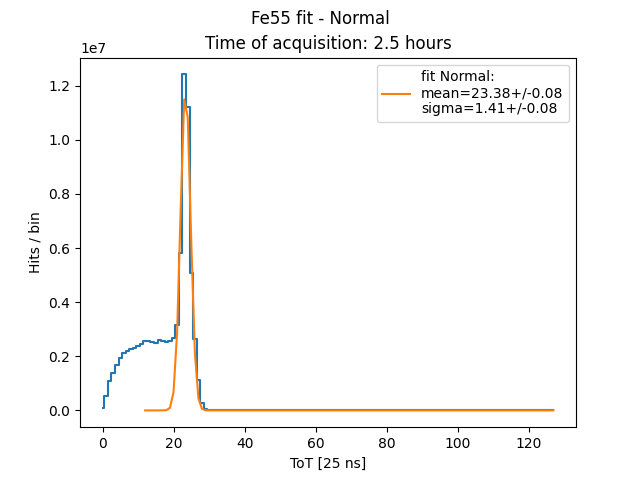
\includegraphics[scale=0.43]{fe55_Normal_peak}}\quad
\subfigure[\textbf{Cascode}3]
{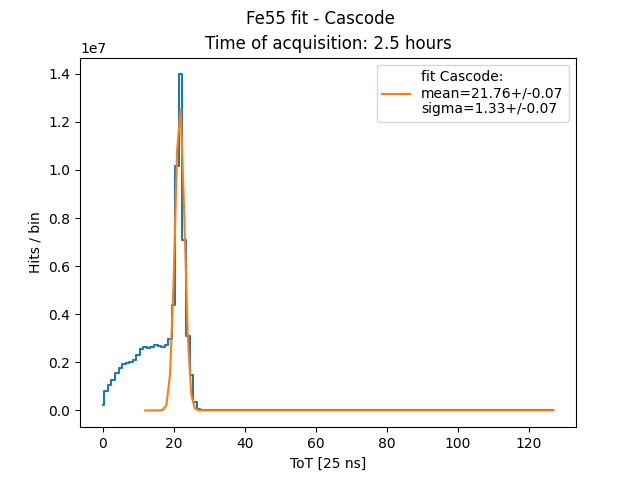
\includegraphics[scale=0.43]{fe55_Cascode_peak}}\\
\subfigure[\textbf{HV Cascode}]
{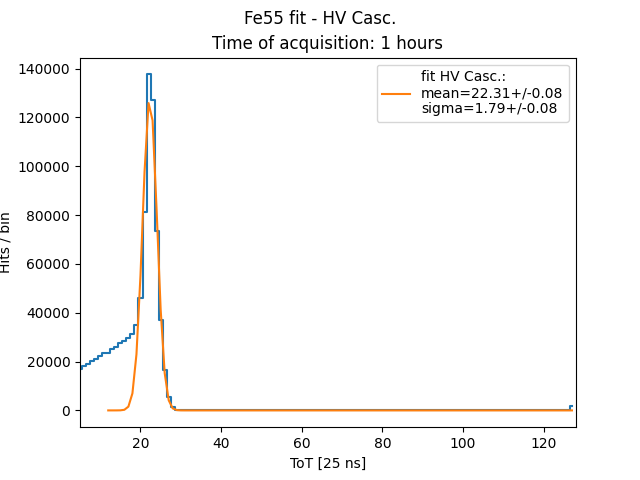
\includegraphics[scale=0.43]{fe_HV Casc._peak}}\quad
\subfigure[\textbf{HV}]
{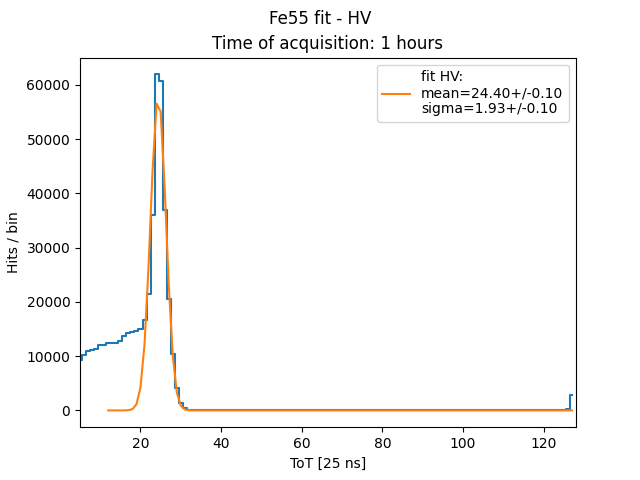
\includegraphics[scale=0.4]{fe_HV_peak}}\\
\caption{\ch{^{55}Fe} single pixels TOT spectrum for all frontends.}
\label{fig:fe_all}
\end{figure}

The TOT spectra of single pixels in each of the four flavors are reported in~\autoref{fig:fe_all}. The peak corresponds to events where the $\gamma$ interacts close to the collection diode and the entire signal is on a single pixel. The shoulder at smaller TOT is due to the charge only partially collected on a single pixel, since charge is shared among several pixels and no cluster reconstruction is done in this analysis. The TOT peak was fitted by a gaussian function, limited in the region of the peak itself, and the results of the fit are reported in the box of each plot. As it can be seen, for both the HV frontends a cut has been applied at low TOT, only to make clearly visible the emission line, since a lot of noisy pixels caused a sharp peak at zero TOT value. In those flavors there were several columns of not-functioning pixels. 

The TOT peak value can be converted to signal in DAC unit, using the fitted calibration curve TOT vs $Q_{inj}$[DAC] of \autoref{eq:fit_function}, and then converted to signal in electrons, assuming the nominal conversion factor K of \SI{10.1}{e^{-}/DAC} of \autoref{eq:conversion_factor}. In this way we could see a reasonable agreement between the expected signal $Q_{\SI{5.9}{KeV}}$~=~1616~$e^{-}$ and the measured one for the Normal FE (1610~$e^{-}$) and Cascode FE (1611~$e^{-}$). On the contrary, we observed a significant loss in the collected signal for the HV flavours as expected, due to the AC coupling and the effect of the parasitic capacitance at the sensitive input node. The signal collected was of about 874~$e^{-}$ in the HV normal FE, and 843~$e^{-}$ in the HV Cascode, corresponding to a loss of about 46\% and 48\%, thus improving from previous version of the chip,  where higher loss (> 50\%) were found.

This signal loss is not obvious from the TOT spectra, since in the HV FEs the measured threshold was lower (\autoref{tab:th_noise_all}) with respect to the Normal and Cascode FE. So even if the collected charge is smaller (approximately half), and the TOT signal is smaller than expected from the calibration curve (\autoref{fig:totfit_cut}), the lower threshold does not allow to make the difference evident.

%--------------------------------------------------------------------
\subsection{\ch{^{241}Am}}

%AGGIUNGI REFERENZA (GAMMA RAY SPECTRUM OF AM-241 IN A BACK SCATTERINGGEOMETRY USING A HIGH PURITY GERMANIUM DETECTOR)

The \ch{^{241}Am} source has a more complex spectrum (\autoref{fig:am241_spectrum}) and not all of its peaks can be detected by the chip (because of the limited TOT range available). The spectrum shows other minor peaks besides the usual intense gamma peaks (59.5 and \SI{26.3}{KeV}) and several characteristic L X-rays from \ch{^{237}Np} (20.7, 17.7 and \SI{13.9}{KeV})~\cite{terada2016measurements}.\\ 

\begin{figure}[h!]
\centering
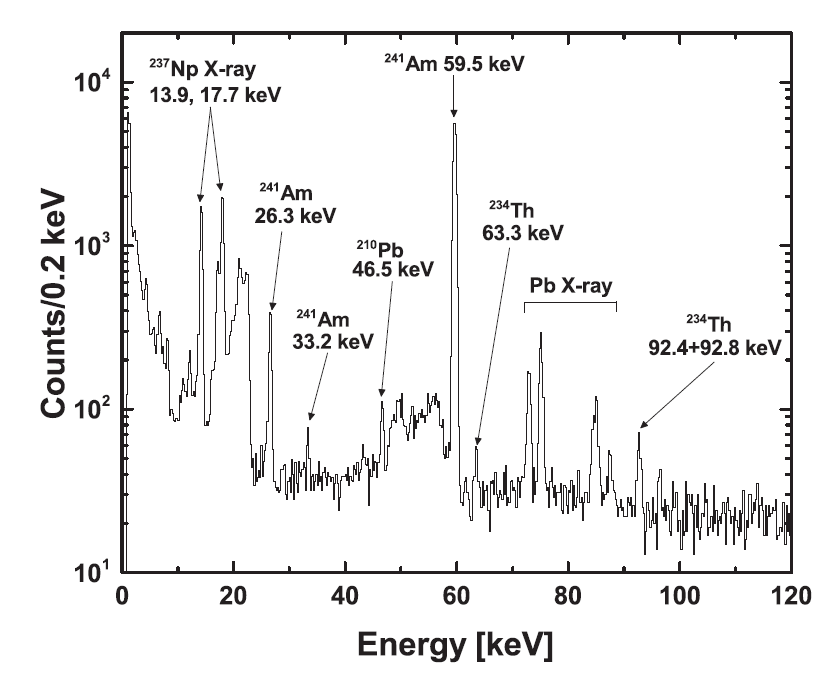
\includegraphics[scale=.6]{Am241_2}
\caption{\ch{^{241}Am} $\gamma$ emission spectrum. From~\cite{terada2016measurements}.}
\label{fig:am241_spectrum}
\end{figure}

The measured TOT spectra obtained with the \ch{^{241}Am} source emitting on the four flavors are reported in~\autoref{fig:am_all}. Two peaks at lower energy are clearly visible while, for higher TOT values there are larger structures. They have been fitted by a distribution given by the sum of an exponential (to characterize the background) and four gaussians for the four visible peaks of the source. Fit results are reported in the box for each plot and the peak mean values for Normal and Cascode FE, together with the peaks obtain with the other sources, are shown in~\autoref{tab:source_conv_norm} and ~\autoref{tab:source_conv_casc}, respectively.

\begin{figure}[h!]
\centering
\subfigure[\textbf{Normal}]
{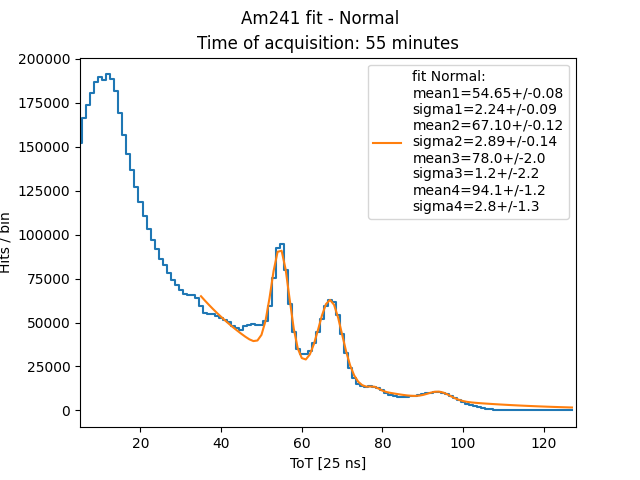
\includegraphics[scale=0.43]{am_Normal_peak}}\quad
\subfigure[\textbf{Cascode}]
{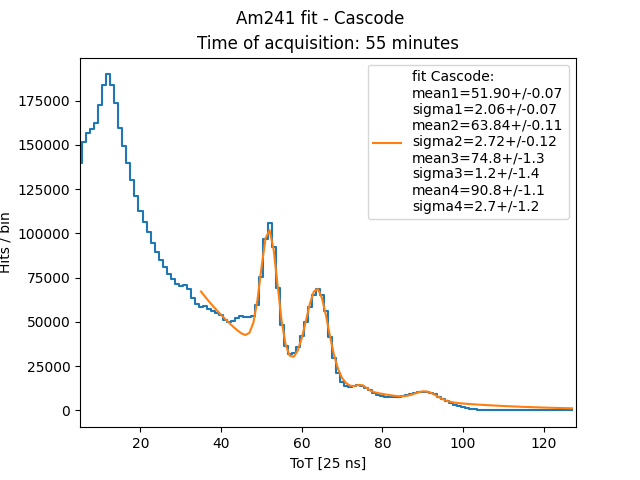
\includegraphics[scale=0.43]{am_Cascode_peak_last}}\\
\subfigure[\textbf{HV Cascode}]
{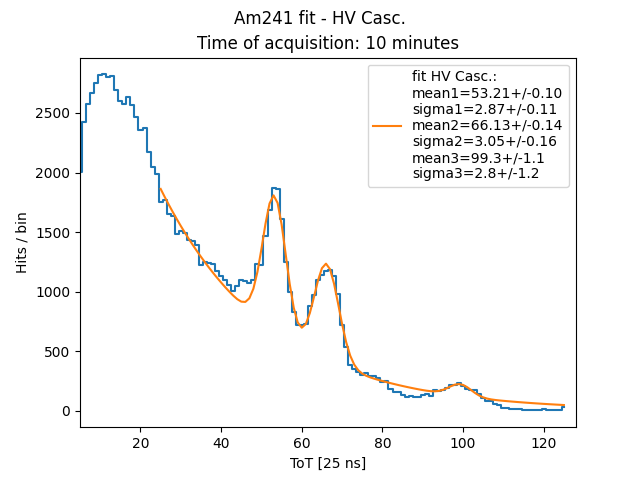
\includegraphics[scale=0.43]{am_HV Casc._peak}}\quad
\subfigure[\textbf{HV}]
{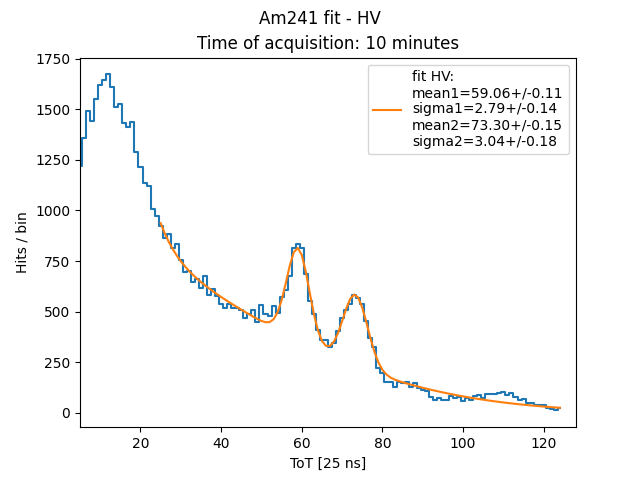
\includegraphics[scale=0.43]{am_HV_peak}}\\
\caption{\ch{^{241}Am} single pixels TOT spectrum for all frontends.}
\label{fig:am_all}
\end{figure}


In the case of the first two flavors, it was possible to fit four peaks of the emission lines. In case of the HV flavors instead, only three peaks for the HV-Cascode FE and two for the HV. It should be noted that in the HV flavors there is a significant (nominal 41.5\%) charge loss as discussed in~\autoref{sec:improved_circuit}. Nonetheless, since the threshold for the HV flavors is much smaller than the one for the Normal flavor (\autoref{tab:th_noise_all}), the peaks appear at roughly the same TOT value.


%As already discussed (\autoref{sec:improved_circuit}) the AC-coupling causes about 41.5\% of signal loss, so they are much less evident and more difficult to fit as isolated peak.

%--------------------------------------------------------------------
\subsection{\ch{^{109}Cd}}

The third source employed was the \ch{^{109}Cd}. This isotope decays in \ch{^{109}Ag} by electronic capture, producing a photon of \SI{22}{KeV} in the transition. The TOT measured spectra with \ch{^{109}Cd} source on the four flavors of the matrix are reported in~\autoref{fig:cd_all}. They have been fitted by summing an exponential distribution to model the background, and a gaussian for the source peak. Fit results are shown in the box of each plot and the value obtained for Normal and Cascode FE are reported in~\autoref{tab:source_conv_norm} and ~\autoref{tab:source_conv_casc}, respectively. 


\begin{figure}[h!]
\centering
\subfigure[\textbf{Normal}]
{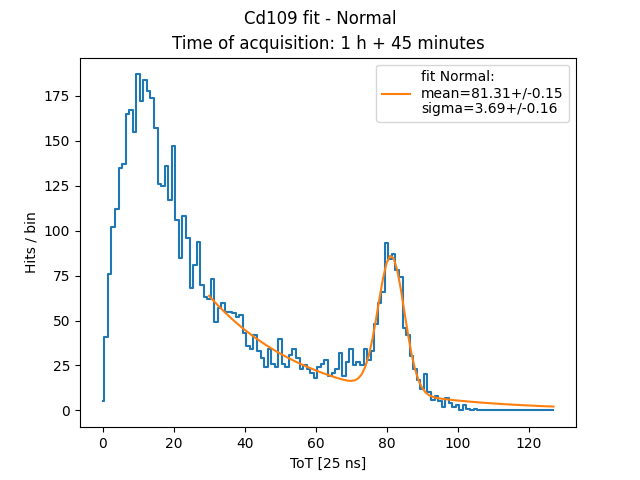
\includegraphics[scale=0.43]{cd109_Normal_peak}}\quad
\subfigure[\textbf{Cascode}]
{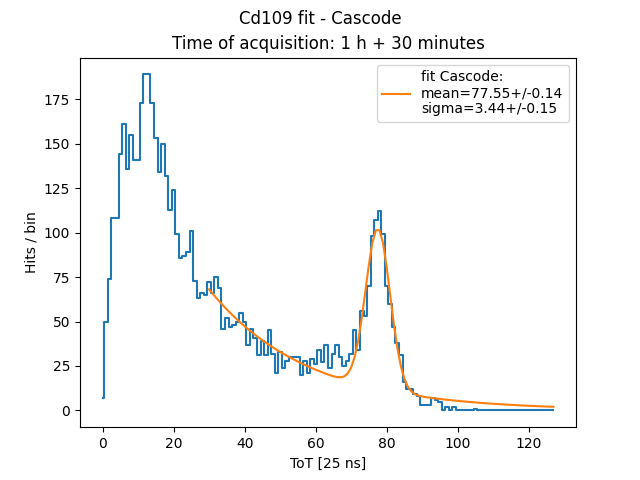
\includegraphics[scale=0.43]{cd109_Cascode_peak}}\\
\subfigure[\textbf{HV Cascode}]
{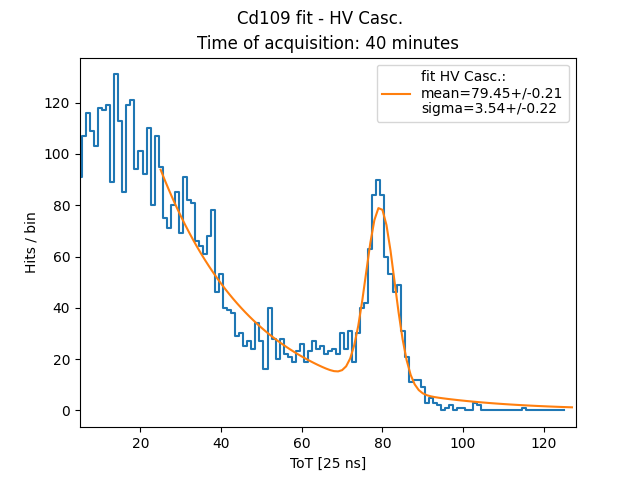
\includegraphics[scale=0.43]{cd109_HV Casc._peak}}\quad
\subfigure[\textbf{HV}]
{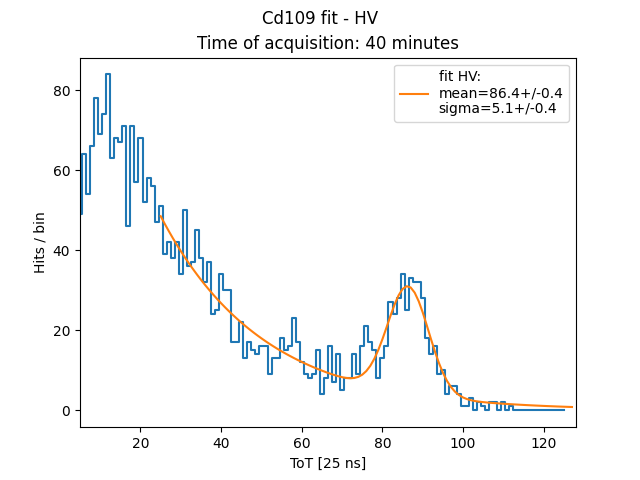
\includegraphics[scale=0.43]{cd109_HV_peak}}\\
\caption{\ch{^{109}Cd} single pixels TOT spectrum for all frontends.}
\label{fig:cd_all}
\end{figure}

As visible from the plots, even in these acquisitions, despite the loss of charge in the HVs, the peaks are measured roughly at the same TOT value due to the lower threshold in these flavors.
\clearpage

%--------------------------------------------------------------------

\subsection{Conversion factor $K$ and $C_{inj}$ absolute calibration}
\label{sec:inj_cap_calib}

The absolute calibration of the conversion factor $K$, that converts a signal charge expressed in DAC units to $e^{-}$, is performed using the data from the \ch{^{55}Fe} source. 
As shown in \autoref{sec:inj_circuit_subsection}, the conversion factor $K$ corresponds to the injected charge given by a voltage step of \SI{1}{DAC} ($\Delta V_{LSB}$~=~\SI{7.03}{\milli V/DAC}) through the injection capacitance $C_{inj}$ implemented in each pixel. 

\begin{equation}
K\bigg(\frac{e^{-}}{DAC}\bigg) = \frac{C_{inj}}{q_{e^{-}}} \cdot \Delta V_{LSB} 
\end{equation}

For the design value of $C_{inj}$~=~\SI{230}{aF} we expect $K$~=~\SI{10.1}{e^{-}/DAC}, but an absolute measurement is needed since there could be significant variations from chip to chip and also across the matrix.

As first step the TOT value of the peak of the \SI{5.9}{KeV} $\gamma$ line for each pixel is converted to signal charge in DAC, $Q_{\SI{5.9}{KeV}}$[DAC], using the fitted calibration curve of~\autoref{eq:fit_function}.

Specifically the fit function was inverted obtaining:
\begin{equation}
x(y) = \bigg(\frac{t}{2} - \frac{b}{2a} + \frac{y}{2a}\bigg) \pm \sqrt{\bigg(\frac{t}{2} + \frac{b}{2a} - \frac{y}{2a}\bigg)^{2} + \frac{c}{a}}
\end{equation}
where \textit{x} represents the charge in DAC corresponding to the TOT labeled by \textit{y}. We have only considered the function with the "+" to model the data, the other has been discarded.

As shown in~\autoref{tab:radio_sources}, the charge released in the sensor by the \SI{5.9}{KeV} $\gamma$ corresponds roughly to $Q_{\SI{5.9}{KeV}}$[$e^{-}$]~=~1616~$e^{-}$. Therefore the conversion factor $K$ for each pixel can be calculated as:
\begin{equation}
K\bigg(\frac{e^{-}}{DAC}\bigg) = \frac{1616 \, e^{-}}{Q_{\SI{5.9}{KeV}}(DAC)}
\label{eq:inj_cap}
\end{equation} 

By these steps, a value of the conversion factor $K$ was estimated for each pixel in the Normal and Cascode FE. The map of the measured values together with their distribution in the two flavors is shown in~\autoref{fig:cap_dist}, with the results of the gaussian fit. In \autoref{tab:cap_mean} the average conversion factors found in the two flavors are compared with the design values, showing a good agreement (10\%).

It is important to stress that due to the signal loss in the HV flavours, the amount of charge collected from \SI{5.9}{KeV} $\gamma$ is not really known thus it is not possible to perform the absolute calibration of the conversion factor for the pixels in these flavours. 

\begin{figure}[h!]
\centering
\subfigure[Normal]
{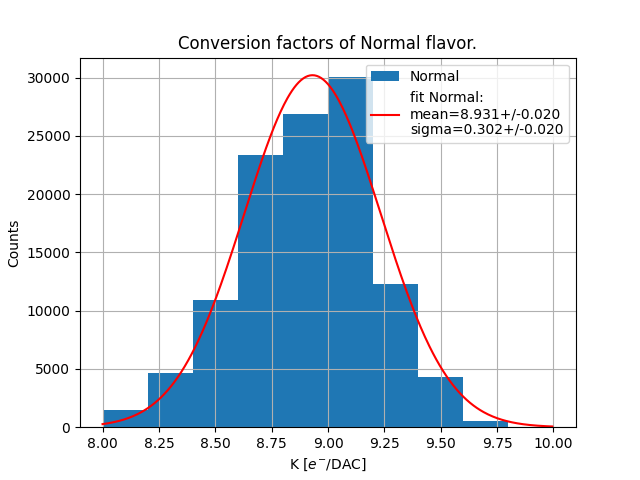
\includegraphics[scale=0.43]{k_fe_Normal_first2}}\quad
\subfigure[Cascode]
{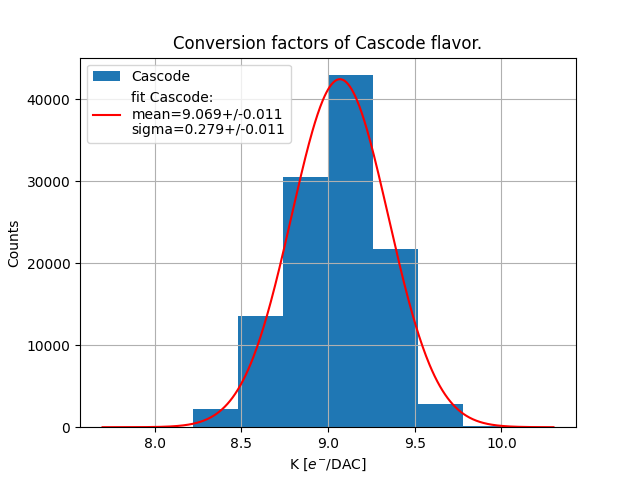
\includegraphics[scale=0.43]{k_fe_Cascode_first2}}\quad
\subfigure[Map of the conversion factors for Normal FE.]
{\includegraphics[scale=0.43]{k_maps_Normal_first2}}\quad 
\subfigure[Map of the conversion factors for Cascode FE.]
{\includegraphics[scale=0.43]{k_maps_Cascode_first2}}\\
\caption{In the first row, the distribution of the conversion factor $K$ measured for all pixels in the Normal and Cascode FE. In the second row the maps of the conversion factor values in Normal and Cascode sectors.}
\label{fig:cap_dist}
\end{figure} 


\begin{table}[h!]
\centering
\begin{tabular}{C{2.8cm}|C{2.5cm}|C{2.5cm}|C{2.5cm}}
\hline
Source peak & $K_{design}$ ($\frac{e^{-}}{DAC}$) & $K_{Normal}$ ($\frac{e^{-}}{DAC}$) & $K_{Cascode}$ ($\frac{e^{-}}{DAC}$)\\[2ex]
\hline
\hline
\ch{^{55}Fe} (5.9 KeV) & 10.10  & 8.93 & 9.07\\[1ex]
\hline
\hline
\end{tabular}
\caption{Average conversion factor $K$ for the Normal and Cascode FE using the \ch{^{55}Fe} radioactive source emission line at \SI{5.9}{KeV}.}
\label{tab:cap_mean}
\end{table}


%--------------------------------------------------------------------
\subsection{Check on calibration curve TOT vs $Q_{inj}$ with radioactive sources}\label{sec:check}

The calibration of the TOT vs $Q_{inj}$(DAC) response with the injection circuit could be performed only up to $\approx$ 170 DAC (about 1700~$e^{-}$). The radioactive sources can be used up to higher energy to check the agreement of the response with the fitted function in~\autoref{eq:fit_function}.\\

This comparison is shown in \autoref{fig:inj_cap_10} and \autoref{fig:inj_cap_sources}. In both plots the TOT vs $Q_{inj}$(DAC) fitted curve is displayed superimposing the points corresponding to each $\gamma$ line from the different sources. 
For each $\gamma$ line the point shown in the plot has the TOT measured from the source spectrum and the charge in DAC corresponding to the charge released by that photon.  
In~\autoref{tab:source_conv_norm} and in~\autoref{tab:source_conv_casc} the various inputs for Normal and Cascode sectors are shown. 
The signal charge in DAC, corresponding to the number of $e^{-}$ of each $\gamma$ line, has been calculated using either the nominal conversion factor equal to 10.1~$\frac{e^{-}}{DAC}$ or the average value of the conversion factor $K$ measured with \ch{^{55}Fe} absolute calibration (\autoref{tab:cap_mean}). 

\begin{figure}
\centering
\subfigure[Normal]
{\includegraphics[scale=0.44]{ToT_Normal_thesis_last}}\quad
\subfigure[Cascode]
{\includegraphics[scale=0.44]{ToT_Cascode_thesis_last}}\\
\caption{TOT vs Q calibration curve measured with the internal injection circuit compared with response from several $\gamma$ lines from radioactive sources, assuming the nominal conversion factor equal to 10.1~$e^{-}$/DAC.}
\label{fig:inj_cap_10}
\end{figure} 


\begin{figure}[h!]
\centering
\subfigure[Normal]
{\includegraphics[scale=0.44]{ToT_Normal_iron_last}}\quad
\subfigure[Cascode]
{\includegraphics[scale=0.44]{ToT_Cascode_iron_last}}\\
\caption{TOT vs Q calibration curve measured with the internal injection circuit compared with response from several $\gamma$ lines from radioactive sources, assuming the conversion factor obtained from \ch{^{55}Fe}.}
\label{fig:inj_cap_sources}
\end{figure} 

In~\autoref{fig:inj_cap_10}, we can see a reasonable agreement between data and TOT fitted function, with the nominal conversion factor, and in case of the Normal FE, a slightly better agreement using the absolute calibration of the conversion factor specific for this chip. 
Deviations from the fitted TOT response are visible, especially in the Cascode FE above \SI{600}{DAC} ($\approx$ 6000~$e^{-}$), and this effect could be ascribed to a deviation from the linear response of the TOT to high signal, more likely to happen in the Cascode flavor that has higher gain.

This preliminary study showed that through the calibration of the TOT with internal injection circuit, and the absolute calibration, we are now able to interpret data from the MIP, collected during the TB,  with a reasonable accuracy to perform the reconstruction, which was the main purpose of this analysis.

\begin{table}[h!]
\centering
\begin{tabular}{C{1.2cm}|C{1.5cm}|C{1.5cm}|C{1.8cm}|C{1.6cm}|C{2.1cm}|C{2.1cm}}
\hline
Source & Energy $\gamma$ [KeV] & $Q_{expected}$ [$e^{-}$] & $ToT_{measured}$ & $Q_{measured}$ [DAC] & Q [DAC]($e^{-}$) \footnotesize{with nominal K factor = 10.1 $e^{-}$/DAC} & Q [DAC]($e^{-}$) \footnotesize{with \ch{^{55}Fe} K factor = 8.93 $e^{-}$/DAC}\\[2ex]
\hline
\hline
\ch{^{55}Fe} & 5.9 & 1616 & 23.4 & 180 & 160 (1820) & 181 (1610) \\[0.5ex]
\hline
\ch{^{241}Am} & 13.9 & 3808 & 54.7 & 429 & 377 (4338) & 426 (3836) \\[0.5ex]
\hline
\ch{^{241}Am} & 17.7 & 4849 & 67.1 & 530 & 480 (5352) & 543 (4733) \\[0.5ex]
\hline
\ch{^{241}Am} & 20.7 & 5671 & 78.0 & 618 & 561 (6242) & 635 (5520) \\[0.5ex]
\hline
\ch{^{109}Cd} & 22 & 6027 & 81.3 & 645 & 597 (6512) & 675 (5759) \\[0.5ex]
\hline
\ch{^{241}Am} & 26.4 & 7233 & 94.1 & 748 & 716 (7558) & 810 (6683) \\[0.5ex]
\hline
\hline
\end{tabular}
\caption{Emission lines of \ch{^{55}Fe}, \ch{^{241}Am}, \ch{^{109}Cd} sources for Normal frontend.}
\label{tab:source_conv_norm}
\end{table}

\begin{table}[h!]
\centering
\begin{tabular}{C{1.2cm}|C{1.5cm}|C{1.5cm}|C{1.8cm}|C{1.6cm}|C{2.1cm}|C{2.1cm}}
\hline
Source & Energy $\gamma$ [KeV] & $Q_{expected}$ [$e^{-}$] & $ToT_{measured}$ & $Q_{measured}$ [DAC] & Q [DAC]($e^{-}$) \footnotesize{with nominal K factor = 10.1 $e^{-}$/DAC} & Q [DAC]($e^{-}$) \footnotesize{with \ch{^{55}Fe} K factor = 9.07 $e^{-}$/DAC}\\[2ex]
\hline
\hline
\ch{^{55}Fe} & 5.9 & 1616 & 21.8 & 178 & 160 (1795) & 178 (1611) \\[0.5ex]
\hline
\ch{^{241}Am} & 13.9 & 3808 & 51.9 & 408 & 377 (4125) & 420 (3704) \\[0.5ex]
\hline
\ch{^{241}Am} & 17.7 & 4849 & 63.8 & 500 & 480 (5053) & 535 (4537) \\[0.5ex]
\hline
\ch{^{241}Am} & 20.7 & 5671 & 74.8 & 585 & 561 (5905) & 625 (5302) \\[0.5ex]
\hline
\ch{^{109}Cd} & 22 & 6027 & 77.6 & 606 & 597 (6118) & 665 (5494) \\[0.5ex]
\hline
\ch{^{241}Am} & 26.4 & 7233 & 90.8 & 708 & 716 (7149) & 798 (6419) \\[0.5ex]
\hline
\hline
\end{tabular}
\caption{Emission lines of \ch{^{55}Fe}, \ch{^{241}Am}, \ch{^{109}Cd} sources for Cascode frontend.}
\label{tab:source_conv_casc}
\end{table}


\clearpage
%--------------------------------------------------------------------
\section{Operation with low threshold} \label{sec:low_thr}
 
Many experimental environments are exposed to high doses of radiations, thus one important target in sensor design is to keep the detection efficiency high even after radiation damage, that could cause a reduction of the collected signal due to trapping. 

For this reason, many tests were performed to understand the chip behaviour at low threshold, that is needed to preserve a good efficiency even with a reduced signal, caused by charge sharing or charge trapping, especially in case of thin epitaxial material.


%--------------------------------------------------------------------
\subsection{Registers optimization}\label{sec:currents}

As we have seen in~\autoref{sec:improved_circuit}, there are many global registers that control the operating point of the front-end circuit and the discriminator threshold as well as the readout sequence. For this reason, it was necessary to first explore their possible settings in order to operate the chip at low threshold.\\

Now we will go through the main registers used for this purpose, to explain their functionality, only focusing on those that affect the threshold and its dispersion.


\begin{itemize}
\label{currents}
\item \textit{$I_{CASN}$} : this current is responsible of the output baseline signal. In particular it sets the baseline of the output signal that goes to the discriminator input. For a given value of the discriminator threshold, set with a different register, the higher \textit{$I_{CASN}$} and the baseline, the lower is the effective threshold. 
%This increase in the baseline also increase a little bit the gain.  
\item \textit{$I_{THR}$}: it controls the pre-amplifier feedback strength and speed, so it is responsible for the output reset rate. With lower $I_{THR}$ the gain increases, so the threshold decreases, according to \autoref{eq:disp_gain}. Lowering $I_{THR}$ also increases the time that the analog output takes to get back to the baseline. As a consequence with lower \textit{$I_{THR}$} also the TOT response changes, increasing a lot the maximum value of the TOT. In fact it is recommended to set $I_{THR}$ to relatively high value (e.g. \SI{8}{nA}~\cite{Moustakas:2021gjr}) in order to avoid high TOT slope and saturation, which limits the TOT resolution.
\item \textit{$I_{DB}$}: this current represents the primary current that sets the discriminator threshold voltage. In threshold tuning (see~\autoref{sec:tuning}) another current is added to this, to fine tune the pixel threshold.
%corresponds to \textbf{$I_{DISC,coarse}$} explained in~\autoref{sec:tuning}, and it
%(\textbf{$I_{DISC,fine}$}$\cdot$TDAC)
\item \textit{$I_{TUNE}$}: 
%it corresponds to \textbf{$I_{DISC,fine}$} (\autoref{sec:tuning}). 
referring to the tuning equation (\autoref{eq:tuning_eq}, in~\autoref{sec:tuning}), this is the current to multiply by the TCODE value (that is the decimal representation of the TDAC value), which is added to $I_{DB}$, during the tuning process.
\item \textit{$I_{BIAS}$}: this current acts on the pre-amplifier input transistor and influences the gain, thus the threshold and its dispersion. In particular increasing this value, the gain increases and the threshold and its dispersion decrease. Nevertheless it cannot be increased too much since it affects the power consumption, too.
\end{itemize}


\begin{comment}
\footnote{
\begin{equation}
I_{DISC} = I_{DISC, coarse} + (TCODE - 1) \cdot I_{DISC,fine},  \hspace{.5cm}	where \hspace{.5cm} 1 \leq TDAC \leq 7
\end{equation}
}
\end{comment}


%ITHR : on chat hung said instead ITHR=64 corresponds to 25 nA and ITHR=20 to 8 nA
%https://confluence.desy.de/pages/viewpage.action?spaceKey=BI&title=VTX+Lab+Set+Up+Operation

%--------------------------------------------------------------------
\subsection{Comparison between data and simulation}

To understand how the registers' setting of the chip influences the threshold, several measurements have been taken with different configuration values.
The results are compared with some simulations done by another researcher (Hung Pham, IPHC in Strasbourg), who participates in the study and characterization of TJ-Monopix2 chip, for the VTX upgrade program.

\begin{description}
\item[\textbf{$I_{CASN}$}] 
\end{description}

In Figure~\autoref{fig:icasn_sim} the simulated behaviour of the threshold depending on the value of $I_{CASN}$ is shown.

%thr_gain_icasn(sim)_last2
\begin{figure}[h!]
\centering
\subfigure[Simulation of threshold values varying $I_{CASN}$.\label{fig:icasn_sim}]{
\includegraphics[scale=.8]{prova2}}\\
\subfigure[Threshold vs. $I_{CASN}$ for $I_{THR}$= 20, 40, \SI{64}{DAC}.\label{fig:alltrends_icasn}]{
\includegraphics[scale=.55]{all_trends(ICASN)_last}}\\
\caption{Simulation and experimental data of threshold vs. $I_{CASN}$, fixing $I_{THR}$.}
\end{figure} 


To verify the trend of the threshold as $I_{CASN}$ varies, three different acquisitions have been taken fixing $I_{THR}$ = 20, 40, \SI{64}{DAC} respectively, and increasing $I_{CASN}$ from 0 to \SI{30}{DAC}, with a step of \SI{5}{DAC}. We have done these measurements enabling about 200 pixels in the Cascode FE. The mean thresholds of the enabled pixels have been measured by the S-curve method for each registers' setting, so the threshold distributions have been fitted with a gaussian function to estimate the average threshold value and its dispersion. Then these values have been converted in electrons unit, using the nominal conversion factor $K$~=~\SI{10.1}{e^{-}/DAC} (\autoref{eq:conversion_factor}).

The results obtained are reported in Figure~\autoref{fig:alltrends_icasn} and they seem to follow the trend of the simulation, despite the few experimental points measured. As a matter of fact, also during these measurements we noticed something strange. Lowering $I_{THR}$, a lot of hot pixels started to fire, not allowing a reasonable measurement. As explained in the previous (\autoref{sec:currents}), decreasing $I_{THR}$, also the threshold decreases, making the pixels hot, due to the aforementioned cross-talk issue, addressed in~\autoref{sec:xtalk}

\begin{description}
\item[\textbf{$I_{THR}$}]
\end{description}

\begin{figure}[h!]
\centering
\subfigure[Simulation of threshold values increasing $I_{THR}$.\label{fig:ithr_sim}]{
\includegraphics[height=5.5cm, width=14cm]{ithr_simulation3_last}}\quad
\subfigure[Threshold vs. $I_{THR}$ for $I_{CASN}$= 0, 5, 10, \SI{15}{DAC}.\label{fig:alltrends_ithr}]{
\includegraphics[scale=.55]{all_trends(ITHR)_last}}\\
\caption{Simulation and experimental data of threshold vs. $I_{THR}$, fixing $I_{CASN}$.}
\end{figure}

Reusing the same data of the previous measurements, the trend of the threshold have been studied, varying the value of $I_{THR}$ and fixing $I_{CASN}$.
In this case, only $I_{CASN}$ from 0 to \SI{15}{DAC} is considered, because for higher values we could not manage to take enough threshold measurements for the cross-talk issue mentioned above. In fact increasing $I_{CASN}$, the threshold decreases, making some pixels hot, and invalidating the measurements.

As expected, increasing $I_{THR}$ results to lower gain so higher threshold, and faster return to baseline. 
We can compare the measured trend, shown in Figure~\autoref{fig:alltrends_ithr}, with the expected one from the simulation shown in Figure~\autoref{fig:ithr_sim}, noting a qualitative agreement between them.


\begin{description}
\item[\textbf{Time Over Threshold (TOT)}]
\end{description}

The last analysis done to make a comparison with the simulations, is about the trend of the TOT changing the value of $I_{CASN}$ for a fixed value of $I_{THR}$ and vice versa. In particular we consider the data obtained with $I_{CASN}$ fixed to \SI{0}{DAC} and $I_{THR}$ to \SI{64}{DAC}, which are the values studied and used for these registers during the Test Beam in Desy.

\begin{figure}[h!]
\centering
\subfigure[Data]
{\includegraphics[scale=0.35]{tot_curves_icasn0}}\quad
\subfigure[Simulation]
{\includegraphics[scale=0.65]{tot_curves_icasn0_simu2_last}}\\
\caption{TOT vs $Q_{inj}$ varying $I_{THR}$, with $I_{CASN}$~=~\SI{0}{DAC} for Cascode FE.}
\label{fig:tot_vs_ithr}
\end{figure}

\begin{figure}[h!]
\centering
\subfigure[Data]
{\includegraphics[scale=0.48]{tot_curves_ithr64}}\\%\quad
\subfigure[Simulation]
{\includegraphics[scale=0.55]{tot_curves_ithr64_simu2_last}}\\
\caption{TOT vs $Q_{inj}$ varying $I_{CASN}$, with $I_{THR}$~=~\SI{64}{DAC} for Cascode FE.}
\label{fig:tot_vs_icasn}
\end{figure}

%Results are reported in~\autoref{fig:tot_vs_ithr} and~\autoref{fig:tot_vs_icasn}. 
The shapes of the measured TOT curves (\autoref{fig:tot_vs_ithr}(a) and \autoref{fig:tot_vs_icasn}(a)) are a little different than those obtained in the simulations(\autoref{fig:tot_vs_ithr}(b) and \autoref{fig:tot_vs_icasn}(b)), in particular at high injected charge. The range of charge explored was limited by the saturation of the charge injection circuit, previously discussed (\autoref{sec:inj_circuit_subsection}).

\newpage
%--------------------------------------------------------------------

\subsection{Low threshold operation, threshold dispersion and tuning} \label{sec:tuning}

After the study on register optimization to operate the matrix at low threshold, we found a stable working point around 250~$e^{-}$, as shown in this section. To reach this global threshold value it was also important to have a uniform threshold distribution across the pixels in the matrix. 

TJ-Monopix2 is equipped with a circuit which allows the \textit{threshold tuning}. We have already mentioned that the analog part of the in-pixel front-end (\autoref{fig:tj2core}) includes the 3-bit threshold tuning DAC, that can be used to adjust the discriminator threshold of each pixel with respect to the global chip threshold level thus reducing the threshold dispersion. In other words it can adjust every pixel threshold, in order to have a threshold on the matrix as uniform as possible, which is especially important to operate the matrix with low threshold, needed with the reduced collection efficiency due to radiation damage.  This system has been designed to compensate for the various effects causing threshold dispersion, related to biasing non uniformity, process and temperature variations, and radiation damage. \\

%
Specifically, the Tuning DAC (TDAC) circuit shown in~\autoref{fig:tdac}, allows the threshold adjustment in each pixel. This component controls the discriminator active load current $I_{DISC}$ which is partially responsible of the pixel threshold (\autoref{fig:tj2_circuit}). It does not generate $I_{DISC}$ but works as an analog multiplexer, which selects one of seven $I_{DISC}$ lines generated by the main 8-bit biasing DAC. So the possible values of the final $I_{DISC}$ is given by the sum of two contributions:

\begin{equation}
I_{DISC, \scriptscriptstyle TCODE}  = I_{DB} + (TCODE - 1) \cdot I_{TUNE},  \hspace{.5cm}	\mbox{where} \hspace{.5cm} 1 \leq TCODE \leq 7 
\label{eq:tuning_eq}
\end{equation}

% \begin{equation}
% I_{DISC} = I_{DISC, coarse} + (TCODE - 1) \cdot I_{DISC,fine},  \hspace{.5cm}	where \hspace{.5cm} 1 \leq TCODE \leq 7
% \label{eq:tuning_eq}
% \end{equation}

%\textbf{$I_{DISC, coarse}$}
%\textbf{$I_{DISC, fine}$}
\textbf{$I_{DB}$} is the current set by the primary value of threshold, resulting from the setting of the main registers that are responsible for it (\autoref{sec:currents}), together with \textbf{$I_{TUNE}$}, which represents the smallest possible increment to add to \textbf{$I_{DB}$} to fine tune the pixel. The other possibilities are multiples of \textbf{$I_{TUNE}$}. 
So \textbf{$I_{DISC, \scriptscriptstyle TCODE}$} is the current selected by the fine tuning step (TDAC) and it depends on the 3-bit tuning code stored in the in-pixel configuration memory.
"TCODE" is the decimal representation of the TDAC code. 

\begin{comment}
For example if the 3-bit DAC are set to "111", the decimal representation is 7 and the fine tuning provide a current $I_{DISC,7}$, which corresponds to the highest threshold. If the 3-bit are set to "001" the corresponding TCODE is 1 and the current $I_{DISC,1}$ is provided, which set the lowest possible threshold around the central value $I_{DB}$. The particular combination "000" instead (TCODE~=~0) masks the single pixel by disabling the discriminator, without affecting the operation of the others.
\end{comment}


\begin{figure}
\centering
\includegraphics[scale=.8]{tuning_b}
\caption{Schematic of 3-bit Tuning DAC (TDAC)}
\label{fig:tdac}
\end{figure}


\subsection{First results from threshold tuning}

%\roman{Add a couple of sentences that summarize how the threshold tuning algorithm works. }

After deciding on the target threshold, the threshold tuning algorithm tries to assign the optimized TDAC value for each pixel, in order to get as close as possible to the target. In this way, the TDAC values obtained for each single pixel are returned.

We tried to apply the fine tuning method to flatten the threshold of some pixels as much as possible. We have considered about 12.000 pixels of the Cascode FE and the results before and after the threshold trimming for the S-curves and threshold distributions are shown in~\autoref{fig:casc_tuning}.


\begin{figure}[h!]
\centering
\subfigure[Cascode FE S-curves untuned]
{\includegraphics[width=.42\textwidth,keepaspectratio]{s-curve_untuned.jpg}}
\subfigure[Cascode FE S-curves tuned]
{\includegraphics[width=.42\textwidth,keepaspectratio]{s-curve_tuned.jpg}}
\subfigure[Cascode FE threshold distribution untuned]
{\includegraphics[width=.4\textwidth,keepaspectratio] {thr_untuned.jpg}}
\subfigure[Cascode FE threshold distribution tuned]
{\includegraphics[width=.4\textwidth,keepaspectratio]{thr_tuned.jpg}}
\caption{Cascode FE before tuning and after tuning comparison.}
\label{fig:casc_tuning}
\end{figure}

\begin{figure}[h!]
\centering
\subfigure[Map of TDAC value with target threshold of $\approx$ 250~$e^{-}$]
{\includegraphics[scale=0.33]{tdac_map}}\quad
\subfigure[Threshold map of tuned Cascode FE]
{\includegraphics[scale=0.53]{th_map_tuned}}\quad
\caption{Maps of tuned Cascode FE.}
\label{fig:casc_maps_tune}
\end{figure}

As we can see the dispersion has been reduced of the 42\% after the tuning and as consequence the estimation of the threshold is also more precise. \autoref{fig:casc_maps_tune} displays the maps of the threshold and of the TDAC values, such as the TCODE value assigned to each pixel, in order to obtain a threshold as uniform as possible. \\





\section{Hot pixels from cross talk issue and mitigation} \label{sec:xtalk}

As previously mentioned, there was something atypical in the S-curves of the HV flavors during average threshold measurements of all FEs: some "hot" pixels started to appear, showing occupancy greater than 1, thus firing more than the number of injected events. 

\begin{figure}[h!]
\centering
\includegraphics[scale=.5]{hot_first_HV}
\caption{HV-Cascode S-curves showing the hot pixels.}
\label{fig:hot_first}
\end{figure}

These extra hits from hot pixels were not simply related to random fluctuations of pixels above threshold due to their noise, since these hot pixels were firing only when there was some digital activity in the matrix, during the readout sequence of other pixels. The same pixels were instead silent, with no extra hits, in case the readout sequence was not activated by other pixels. 

This is visible in \autoref{fig:hot_first}: the region indicated by the red arrow has extra hits from hot pixels and corresponds to events in the matrix where many pixels have real hits from the injection (Qinj~>~THR) and the digital readout is then active. In the region indicated by the blue arrow instead, where Qinj~<~THR, there are no real hits from the injection which activates the readout, and also the hot pixels do not fire.  

The observation that the hot pixels were not firing simply due to their noise fluctuation, was also confirmed with additional acquisition without injection. With a given setting of the threshold the matrix had no hits, indicating that the threshold was high enough to cut to zero the occupancy from noise fluctuation. As soon as the matrix was stimulated with real hits from a radioactive source, several hot pixels started to fire, sending hits just after the event where real hits from the radioactive source were readout. This was an additional confirmation that the spurious hits were correlated with some activity of the readout sequence. 


This behavior compromises the good functionality of the overall matrix response, because these hot pixels flood the readout, giving unreliable results. Furthermore, during the systematic study of different register configurations the presence of hot pixels prevented using certain settings to reach lower global thresholds. For this reason, a detailed investigation has been conducted in order to understand the reasons why the hot pixels start to fire and how to cure them as much as possible.\\ 

Thanks to these tests we could identify the origin of this cross-talk with some coupling of the front-end,  or the input collection diode, with a specific digital signal activated in the entire matrix during the readout sequence.
Using the available timing information for the hits, their Leading edge (LE),  we could study the time correlation of the extra hits with the timing of the various digital signals in the readout sequence, that could be selectively moved changing some readout registers. 

These tests were performed in controlled situation, as shown in the next section,  and the main conclusion is the following:

\begin{itemize}
\item the cross talk coupling is present in all pixels of the matrix. The responsible digital signal is distributed to each pixel during the readout sequence, producing a similar signal pulse in all pixels.
\item this induced or cross-talk signal is anyway producing hits only in pixels with a threshold lower than the induced signal height. For a given setting of global threshold, higher than the induced signal height, some pixels could have a significantly lower threshold,  simply due to threshold dispersion or other reasons, and they behave as "hot" pixels.  
\item also "normal" pixels can become "hot", firing on this induced signal, if their threshold is reduced, either lowering the global threshold setting or reducing their specific threshold by the TDAC threshold tuning.
\end{itemize}


In the following section we describe some of these tests and some attempts to mitigate the issue using different settings/bias.


%\subsection{Hot pixel issue}

%First of all we noticed that in the s-curves oh the HV flavors (e.g. that of HV-Cascode reported in  \autoref{fig:hot_first}), the atypical behavior could be triggered by a digital signal sent to the matrix during the readout activity at low threshold. This consideration is based on two main reasons:

%\begin{itemize}
%\item when the matrix has high threshold, like for Normal and Cascode FE, all pixels seem to behave as expected, without \textit{hot pixels}.\\ Lowering the threshold and running some source acquisitions without any source, no strange behaviour was observed. Acquiring data with a radioactive source instead, even Normal and Cascode FE seem to reveal the same problem. This led to thinking that during the readout of good pixels an induced signal is created which couples with some other pixels, in particular with those at lower threshold with respect to the average value. If the height of this signal exceeds the threshold of the single pixel, it causes some spurious hits, making the pixel ''\textbf{hot}''.

%\item Moreover, always considering the HV Cascode s-curves, it could be noticed that in the region before the threshold ($Q_{inj}$<threshold, pointed by the blue arrow) there isn't an anomalous activity which means that the induced signal is not due to the BCID tha is always sent to the matrix during the injection or an acquisition with the source, regardless of being above or below the  threshold. The atypical behaviour indeed, is in the region above the threshold ($Q_{inj}$>threshold, pointed by the red arrow) where the occupancy of some pixels becomes greater than 1. This means that these \textit{hot pixels} detect more hits of those injected.

%\end{itemize} 



%From these first observations, we have reached the conclusion that the cross talk could be tied to the readout activity. So we have started investigating the timestamp of those hits not synchronize with the timestamp of the injection.


\subsection{Hot pixel studies}


At first, the threshold has been lowered in order to "create" hot pixels also in the first two flavors of the matrix. In fact, with the TB settings, the threshold for Normal and Cascode FE was higher (above 500~$e^{-}$) than the threshold in the HV FEs (of about 350~$e^{-}$) where the hot pixels were first observed, so the hypothetical induced signal did not cause spurious hits in the two first flavors. For this purpose, different settings were tried, changing some registers responsible for the threshold like those listed and explained in~\autoref{currents}. 
We confirmed that hot pixels were also appearing in the first two flavors, operating the matrix at a global threshold below 350~$e^{-}$. 

Then several tests have been performed under controlled conditions:
\begin{itemize}
\item one healthy (good) pixel was injected;
\item one hot pixel (two or three in different tests) was enabled but not injected;
\item all the matrix except these pixels was disabled.% to prevent other hot pixels' hits from disturbing the readout.
\end{itemize}

\begin{figure}[h!]
\centering
\includegraphics[scale=0.6]{cross_talk_read2}
\caption{Hot pixel study: readout sequence.}
\label{fig:hot_pixel_readout}
\end{figure}


\begin{comment}
\begin{figure}[h!]
\centering
\includegraphics[width=.9\textwidth,keepaspectratio]{cross_talk_redout.jpg}
\caption{Hot pixel study: readout sequence.}
\label{fig:hot_pixel_readout}
\end{figure}
\end{comment}

In this way the readout cycle, shown schematically in \autoref{fig:hot_pixel_readout}, has a known duration, and the timing of the various digital control signals (\textsc{freeze}, \textsc{read}) has a known position with respect to Trailing Edge (TE) of the first hit which activates the readout. The digital readout signal timing can be moved acting on specific registers listed in \autoref{tab:ro_registers}. We studied in detail the time correlation of the hot pixels LE and TE with the digital signals.

Two different timing information have been used to study the time correlation of the induced signals with the digital signals:

\begin{itemize}
\item $\Delta$TS (TimeStamp) between two consecutive hits: the timestamp is assigned by the FPGA when the \textsc{token} rises on the TE of the first hit to read, but only if the previous readout frame is completed. Therefore, if the hit coming from a hot pixel is after the hit from the injected one, the minimum $\Delta$TS has to be equal to the readout time of 1 pixel and so to the duration of the \textsc{freeze} signal.\\
This information has allowed to verify whether the hot pixel fires immediately after the good injected one or not.
\item LE(hit) - TE(previous hit): this quantity measures the elapsed time between the start of a hit (Leading Edge) and the end of the previous one (Trailing Edge). The TE of the first hit  activates the readout and also corresponds to the beginning of the entire readout sequence. All other readout control signals have a known/selectable timing position with respect to this TE. Thus the distance LE(hit) - TE(previous hit) allows to correlate the LE of the spurious hit, due to cross-talk, with the specific digital signal edge that produces the effect. 
This quantity is shown in \autoref{fig:hot_pixel_readout}
for the two cases of hot pixels firing on the rising or falling edge of the \textsc{freeze} signal.
\end{itemize}

%Moreover, since the LE and TE are measured with a 7-bit BCID counter distributed the matrix during its activity, it was important to keep short (<128 clock cycle) the duration of the full readout sequence and to not enable too many pixels in order to not extend too much the readout frame. Otherwise the information on the leading edge of the pixel could not be correlated with the token of the previous hit. In other words, if the readout frame exceed 128 clock cycles, since the token could be raised if the matrix is \textbf{not} freeze, even if an hit is arrived before it could be read only in the next frame when it could rise again the token, but in this case it will have different TimeStamp. So in this case the TS is useless for our purpose.


\subsection{Digital signal responsible for cross talk }

Referring to the readout sequence, in order to understand which digital signal could induce cross-talk, we moved the registers used to control the timing of the these signals with respect to the start of the readout sequence (i.e. with respect to the TE of the first hit). Thus we expected to see the same shift in the LE-TE distance when the responsible digital signal was changed.

\autoref{tab:ro_registers} shows an example of the settings used for these registers. With a timestamp frequency of \SI{40}{MHz}, one clock cycle corresponds to \SI{25}{ns}. 

%This step of the procedure is tied with the necessity to keep the readout sequence within the maximum 128 BCID range.\\

\begin{table}[h!]
\centering
\begin{tabular}{C{5cm}|C{3cm}}
\hline
\hline
Register & Value (clock cycles) \\
\hline
\hline
\textsc{FREEZE\_START\_CONF} & 10\\[0.3ex]
\hline
\textsc{READ\_START\_CONF}& 13 \\[0.3ex]
\hline
\textsc{READ\_STOP\_CONF} & 15 \\[0.3ex]
\hline
\textsc{LOAD\_CONF} & 30 \\[0.3ex]
\hline
\textsc{FREEZE\_STOP\_CONF} & 31\\[0.3ex]
\hline
\textsc{STOP\_CONF} & 31\\[0.3ex]
\hline
\hline
\end{tabular}
\caption{Register values of the readout cycle.}
\label{tab:ro_registers}
\end{table}

For example, if the register \textsc{FREEZE\_START\_CONF}, which is the rising edge of the \textsc{freeze} signal, is responsible for the cross-talk, we expect that shifting its value by a certain number of clock cycles would also delay the timing of the cross-talk induced hit by the same number of clock cycles, and this should be visible in the LE-TE position. \\

%the hot pixels start to fire after that this signal arises due to the hit on the injected pixel. So the value of LE-TE has to be \textsc{FREEZE\_START\_CONF} + some potential delay. Same argument for the other registers. \\

With this procedure, repeated for each readout register, we have confirmed that the cross-talk is related to the rising and falling edge of the \textsc{freeze} signal. In the following examples, one pixel is injected (217,140) and two pixels are enabled (218,155) and (222,188), while the rest of the matrix is disabled.

%In~\autoref{fig:xtalk} an example of some results obtained is displayed.
\begin{figure}[h!]
\centering
\includegraphics[scale=0.8]{xtalk_time}
\caption{An example of the time information used.}
\label{fig:xtalk_tab}
\end{figure}

In~\autoref{fig:xtalk_tab} an example of the time information used is shown, where the timings of the injected pixel are green coloured, that of the hot pixels are white. The quantities reported in the columns of the table are: the row and the column of the hit pixel, the LE and the TE of the hit, the difference between the LE of the hit and the LE of the previous one ($\Delta$LE), the difference between the TE of the hit and the TE of the previous one ($\Delta$TE), the difference between the timestamps of the same consecutive hits ($\Delta$TS), and the timestamp of the hit. All these quantities are expressed in clock cycles. Each row shows a hit coming from the enabled pixels.

In the first two rows (green), two hits of the injected pixel (114,217) are displayed. Their timestamps are different, and the $\Delta$TS~$\approx$~5600 clock cycles can be attributed to the time between two injections. The timestamp is assigned by the FPGA when the \textsc{token} rises on the TE of the first hit to read. 

The hits of the two hot pixels (155,218) and (188,22) (third and fourth row respectively), have TOT~$\approx$~0, thus the LE coincides with the TE, and their timestamps are the same, so they fire at the same time. In particular, the $\Delta$TE of the first hot pixel is 35 clock cycles, which means that it fires during the readout of the previous injected hit (longer blue arrow in~\autoref{fig:hot_pixel_readout}). In this case the $\Delta$TE corresponds to the time elapsed between the TE of the injected hit and the LE of the hit coming from the hot pixel, for which TE~$\simeq$~LE. For the same reason, the zero $\Delta$TE of the hit in the fourth row corresponds to the time elapsed between the two hot pixels' hits, which means that they fire at the same time, due to the same cross-talk induced signal (due to the TE of the \textsc{freeze}).
The hit in the fifth row has a different timestamp with respect to the previous one, but they differ from 55 clock cycles, which means that this hot pixel fires again during the readout of the two previous hit (specifically after the TE of the \textsc{freeze}). 

\begin{figure}[h!]
\centering
\includegraphics[scale=0.4]{xtalk_hist}
\caption{An example of the LE(hit)-TE(previous hit) histogram.}
\label{fig:xtalk}
\end{figure}

\autoref{fig:xtalk} shows the histogram of the elapsed time between the leading edge LE of an hit and the trailing edge TE of the previous hit, when one pixel is injected and two additional hot pixels are enabled. When only one hit is readout, the duration of the \textsc{freeze} signal is of 21 clock cycles. 

\begin{comment}
\begin{figure}[h!]
\centering
\subfigure[An example of the time information used.]
{\includegraphics[scale=0.8]{xtalk_time}}\quad
\subfigure[An example of the LE(hit)-TE(previous hit) histogram.]
{\includegraphics[scale=0.4]{xtalk_hist}}\\
\caption{Some results of the cross-talk studies.}
\label{fig:xtalk}
\end{figure}
\end{comment}





It is possible to see several peaks in the LE(hit) - TE(previous hit) distribution (referring to the readout setting reported in~\autoref{tab:ro_registers}):

\begin{itemize}
\item a peak at 0 clock cycle, representing the event where both hits come from the two hot pixels firing simultaneously after the injection in the other pixel. This means that they are both activated by a given signal and so, it is the most important confirmation that they come from cross-talk and not from a random firing pixel signal;
\item a peak at $\approx$ 18 clock cycles equal to the FREEZE\_START\_CONF value  (10 clock cycles) + 8 clock cycles $\rightarrow$ the rising edge of the \textsc{freeze} signal is responsible for the induced signal;
\item a more pronounced peak at $\approx$ 35 clock cycles equal to the FREEZE\_STOP\_CONF value (31 clock cycles) + 4 clock cycles $\rightarrow$ the falling edge of the \textsc{freeze} signal is also responsible for the induced signal with higher probability than the \textsc{freeze} rising edge;
\item a peak at $\approx$ 55 clock cycles equal to the \textsc{freeze} falling edge (located at 51 clock cycles when 2 different hits are readout in the same sequence) + 4 clock cycles. In more detail, after the first 30 clock cycles until the first LOAD\_CONF, an additional pixel reading starts and it takes another 20 cycles (LOAD\_CONF - FREEZE\_START\_CONF) + 1 cycle to conclude the frame. Therefore, when two pixels are read, the \textsc{freeze}  falls after 51 clock cycles as indicated above, and it is compatible with the last peak in the plot.
\end{itemize}

An additional confirmation of the previous studies, that indicate the \textsc{freeze} as responsible for this cross-talk, was also found by directly observing through the oscilloscope the behaviour of the analog output of a test pixel, available for debugging purpose.    
In~\autoref{fig:analog_xtalk} an analog acquisition of the readout signals is shown, taken during the test performed in a similar way as before. 

\begin{figure}[h!]
\centering
\includegraphics[scale=.6]{xtalk_analog}
\caption{Cross-talk of the \textsc{FREEZE} signal on oscilloscope's analog output, for different value of \textsc{FREEZE\_START\_CONF} register.}
\label{fig:analog_xtalk}
\end{figure}

In these tests the analog pixel, together with another pixel in the matrix, was injected with variable signals from 0 to \SI{140}{DAC} (this can be seen by the increasing signal height in the acquisition). Two different groups of spikes are also visible in the analog output: the first and smaller one represents the cross-talk effect on this pixel from the raising of the \textsc{freeze} signal during the readout sequence of the other pixel, while the second, larger one corresponds to the cross-talk from the falling edge of the same signal.
Moreover, it is possible to see that in the two different pictures, the cross-talk induced signals move according to the different settings of the \textsc{FREEZE START/STOP} edge that was changed in the two acquisitions.

As already stated, we run several tests varying the number of pixels to read and the value of the readout registers, using different combination of hot and good pixels and also different spatial location of them in the matrix to exclude the possibility that the problem was related to particular columns. All results are in agreement with the interpretation explained above.\\


\subsection{Cross talk signal height}

%LOGBOOK 15.11.2022

We also tried to estimate the induced signal height from the threshold of the hot pixel. For this purpose, we have tried different settings of the registers cited above, to make a pixel "hot" in order to understand when the induced signal went above the threshold. We have found that the induced signal correspond to about 100/150~$e^{-}$ depending on the bias condition.

An example of these tests is shown in~\autoref{fig:making_hot}. We enabled part of the matrix (the columns 217 and 218 and the rows between 120 and 220), injecting only one pixel (217, 140). In~\autoref{fig:making_hot}(a) the S-curves of different pixels are shown and among these we chose one that was not hot (218, 123).

\begin{figure}[h!]
\centering
\subfigure[$I_{DB}$=100, $I_{TUNE}$=53 - Good behavior for the pixel (218,123) (the red one) with THR~>~\SI{35}{DAC}=350~$e^{-}$, while other pixels with THR$\approx$\SI{15}{DAC}=150~$e^{-}$ are already "hot" ]
{\includegraphics[scale=0.35]{making_hot1}}\quad
\subfigure[$I_{DB}$=60, $I_{TUNE}$=150 - The pixel (218,123) has THR around \SI{20}{DAC} and starts to misbehave]
{\includegraphics[scale=0.35]{making_hot3}}\\
\subfigure[$I_{DB}$=55, $I_{TUNE}$=150 - The pixel has THR below \SI{15}{DAC} and becomes "hot"]
{\includegraphics[scale=0.35]{making_hot2}}\\
\caption{S-curve of the pixel (218, 123) for different register settings, used to gradually reduce its threshold.}
\label{fig:making_hot}
\end{figure}

The S-curves of the same pixel (218, 123) are shown for different register settings used to gradually reduce its threshold. The pixel that has a normal S-curve when it has a high threshold of approximately 350~$e^{-}$ (\autoref{fig:making_hot}(a)), starts to misbehave with occupancy slightly higher than 1 for threshold of about 200~$e^{-}$ (\autoref{fig:making_hot}(b)), and becomes hot for threshold of about 150~$e^{-}$ (\autoref{fig:making_hot}(c)).
We can notice a structure in the S-curve of the hot pixels when the occupancy becomes greater than 1. We did not investigate further this behaviour. 



\subsection{Cross talk mitigation}

As seen in the previous, the hot pixel problem is related to the induced signal produced during the readout, which causes cross-talk. This becomes even more serious when there is a larger threshold dispersion, since although the global threshold is set well above the level of the induced signal, some pixels can still have a threshold lower than the induced signal.

Potentially every pixel could become "hot" if its threshold is lower than the height of the cross-talk signal, since the \textsc{freeze} in sent across the entire matrix. 


\begin{description}
\item \textbf{Threshold trimming}
\end{description}
 
Therefore, a possible treatment could be related to the threshold tuning, explained in~\autoref{sec:tuning}, which could allow to make the pixel thresholds more uniform (smaller threshold dispersion) and at the same time to target a value higher than the induced signals.

\autoref{fig:tuning_hot} shows an example of the results obtained.

\begin{figure}[h!]
\centering
\subfigure[Threshold distribution before tuning procedure.]
{\includegraphics[scale=0.35]{before_tuning}}\quad
\subfigure[Threshold distribution after tuning procedure.]
{\includegraphics[scale=0.35]{after_tuning}}\\
\caption{Threshold tuning to reduce hot pixels.}
\label{fig:tuning_hot}
\end{figure} 

The reduction of the tail in the threshold distribution is evident, in fact the dispersion is reduced by 56\%. The number of the hot pixels also decreases from 18\% to 1.2\% of the total pixels studied. We can also notice that the peak at 0 threshold disappears, which comes from those hot pixels with low thresholds, whose S-curve is so distorted that its threshold evaluation is 0. The hot pixels are those with occupancy greater than 1 and an example of a hot pixel (218,155) with threshold 0 is shown in~\autoref{fig:zero_thr}. After the tuning their thresholds are increased, preventing them from misbehaving.

\begin{figure}[h!]
\centering
\includegraphics[scale=.55]{zero_thr2}
\caption{An example of a hot pixel (218,155) with threshold 0.}
\label{fig:zero_thr}
\end{figure} 



\begin{description}
\item \textbf{Bias Voltage}
\end{description}

Moreover, we have tried to increase the bias voltage of the  matrix to study how it might affect the cross-talk. All previous tests have been performed with $P_{WELL}/P_{SUB}$ set to \SI{-3}{V}. This value was increased to \SI{-6}{V} and there were some improvements. In fact increasing the bias, we expected a decrease of the diode capacitance thus higher gain and lower threshold dispersion. In addition the coupling with the cross-talk signal seemed reduced too and so the induced signal height. \\
\autoref{fig:bias_comp} shows a comparison between the threshold distributions respectively at \SI{-3}{V} and \SI{-6}{V}, with the same register setting and without tuning.

\begin{figure}[h!]
\centering
\subfigure[Threshold distribution at $P_{WELL}/P_{SUB}$~=~\SI{-3}{V}.]
{\includegraphics[scale=0.35]{th_dist_3V}}\quad
\subfigure[Threshold distribution at $P_{WELL}/P_{SUB}$~=~\SI{-6}{V}.]
{\includegraphics[scale=0.35]{th_dist_6V}}\\
\caption{A comparison between the threshold distributions resulted with different biasing voltage, without tuning.}
\label{fig:bias_comp}
\end{figure}

At higher bias voltage not only the threshold is lower (higher gain), but also its dispersion is, as expected. And despite that, there are fewer hot pixels: 1.3\% at \SI{-6}{V} against 17\% at \SI{-3}{V}. Also here, the reduction of the threshold distribution tail is evident. 

\subsection{Conclusion from cross talk studies}

The results obtained with both the threshold tuning and a bias voltage of $P_{WELL}/P_{SUB}$~=~\SI{-6}{V} are shown in~\autoref{fig:bias_tuning}, where we can see the decrease in threshold dispersion with the number of the hot pixels.

\begin{figure}[h!]
\centering
\subfigure[Threshold distribution at $P_{WELL}/P_{SUB}$~=~\SI{-6}{V} without tuning.]
{\includegraphics[scale=0.35]{xtalk_6V_no_tuning}}\quad
\subfigure[Threshold distribution at $P_{WELL}/P_{SUB}$~=~\SI{-6}{V} with tuning.]
{\includegraphics[scale=0.35]{xtalk_6V_tuning}}\\
\caption{A comparison between the threshold distributions at \SI{-6}{V} bias voltage without tuning (a) and with tuning (b).}
\label{fig:bias_tuning}
\end{figure}

%As we can see in~\autoref{fig:bias_tuning}, the threshold dispersion decreases together with the number of the hot pixels. 
In fact, without the tuning there are 1.3\% of them, while after the tuning procedure there are none.

After these tests, we could conclude that with a bias voltage of \SI{-6}{V} and threshold tuning it was possible to operate the matrix with a global threshold of approximately 200/250~$e^{-}$, much higher of the expected minimum threshold of 100~$e^{-}$ (\autoref{tab:tj2_spec}) indicated by the simulations done during the TJ-Monopix2 design, but still totally acceptable to keep a good detection efficiency even after irradiation. 

These cross-talk studies were also crucial to indicate possible mitigation strategies for the next OBELIX chip. 
The origin of the this cross-talk coupling is still under investigation with detailed simulations of the matrix behaviour. At the same time in OBELIX we plan to increase the range of the threshold tuning DAC in order to have the possibility to selectively increase the pixel threshold that are in the tail of the threshold distribution and could otherwise become hot and disturb the readout. 

It should be also noted the cross-talk charge injection happens during the readout and therefore does not affect the charge collected by pixel hit by real particles.

%LOWERING ITHR DECREASED THE INDUCED SIGNAL, BUT MATRIX NOT GOOD FUNCTIONALITY?
%VRESET(agisce sulla dispersione) AND IBIAS(aumenta gain e diminuisce dispersion ma aumenta power consumption)



\begin{comment}
Suggestions from OBELIX meeting.

Probably the coupling is linked to digital power. 
Not from the bulk: +4 clk seems to be the indication for not a direct coupling

Since the distribution of the power is from the edge,  first and last column should be more solid against this effect and hot pixel should be more present in the center? 
They asked if we have a  map of the hot pixels

Also suggested to change the clock and see if the delay from the FREEZE edge is at the same delay or not. 

\end{comment}




\section{Test Beam results}

The full characterization of the chip allowed to interpret data collected during the Test Beam campaign at Desy (June 2022). Several tests have been conducted to study the electrical characteristics and the hit detection efficiency of the unirradiated modules \cite{Bespin:2023vyw}.

\bigskip

\textbf{Experimental apparatus and DUTs}

\medskip

\begin{figure}[h!]
\centering
\includegraphics[scale=.6]{TBJUNE22_2}
\caption{Test Beam experimental apparatus.}
\label{fig:tb}
\end{figure}

The measurements have been performed using an electron beam with energies in the range of 3-\SI{5}{GeV}, at DESY II testbeam facility at DESY, Hamburg \cite{Diener:2018qap}. The experimental apparatus consisted of a beam telescope, a Trigger Logic Unit to provide trigger and control signals employed during test beams, a scintillator trigger and a rotation-translation stage on which install the device under test. (~\autoref{fig:tb}).


\begin{comment}
\begin{figure}[h!]
\centering
\subfigure[Test beam apparatus.]
{\includegraphics[scale=0.8]{TBJUNE22_PHOTO}}\quad
\subfigure[Test beam schematics.]
{\includegraphics[scale=0.8]{TBJUNE22}}\\
\caption{Test Beam setting at DESY.}
\label{fig:tb}
\end{figure}
\end{comment}

Three different modules have been tested with different sensor geometries, among which the chip W14R12 that we have studied in depth through laboratory measurements. All results described in previous sections have been crucial to interpret data obtained during these tests. Preliminary setting were used (\autoref{tab:tb_settings}), featuring high threshold ($\approx$500~$e^{-}$).

We will briefly describe the results obtained in the following \cite{BelleIIVTXUpgradeGroup:2023isk}.

\bigskip


\textbf{Cluster charge distribution and efficiency measurements}

\medskip

The cluster distribution obtained from electron beam measurements is shown in Figure~\autoref{fig:clust_dist}. 
This distribution was fitted by a Landau function and the signal of each pixel was corrected by a calibration factor, which we have discussed in depth in~\autoref{sec:inj_cap_calib}.
The MPV of the cluster charge was obtained from the fit, resulting in (3010$\pm$24)~$e^{-}$, which is in line with the calculated deposited energy of about $\approx$ (3200$\pm$194)~$e^{-}$.\\


\begin{figure}[h!]
\centering
\subfigure[\label{fig:clust_dist}Cluster charge distribution.]
{\includegraphics[scale=0.65]{cluster_dist}}\quad
\subfigure[\label{fig:det_eff} (99.54$\pm$0.04)~\% hit detection efficiency of DC-coupled flavours at \SI{3}{V} bias voltage.]
{\includegraphics[scale=0.6]{det_eff_DC}}
\end{figure}

\begin{comment}
\begin{figure}
\centering
\includegraphics[scale=.7]{cluster_dist}
\caption{Cluster charge distribution.}
\label{fig:clust_dist}
\end{figure}
\end{comment}


The hit detection efficiency $\epsilon$ is evaluated by the ratio of the matched hit to the total tracks. For the DC-coupled flavors, for a threshold of $\approx$  500-600~$e^{-}$ (\autoref{tab:th_noise_all}), the hit efficiency measured is 99.54$\pm$0.04~\%, as shown in Figure~\autoref{fig:det_eff}. This result will be compared with the efficiency of the irradiated chip, to test the  good efficiency performance even after irradiation.\\

In the next phase the sensors have been irradiated ranging from \num{e14} to \SI{e15}{n_{eq}/cm^{2}}, and in a new test beam campaign in July 2023, the chip response have been examined under these conditions.


%2023??

\begin{comment}
\begin{figure}
\centering
\includegraphics[scale=.7]{det_eff_DC}
\caption{(99.54$\pm$0.04)~\% hit detection efficiency of DC-coupled flavours at \SI{3}{V} bias voltage.}
\label{fig:det_eff}
\end{figure}
\end{comment}




\begin{comment}
Initially a depletion depth study have been done and with a voltage bias of -3 V (Normal and Cascode FE), for the chip W14R12 resulted 33$\mu$m $\pm$ 0.04 (stat.) $\pm$ 2.53 (sys.).

Voltage scan measurements have been performed for both the two type of pixel couplings, such as DC and AC coupled. For the latter, only some first results have been obtained. 

\begin{description}
\item[Normal FE]
\end{description}

In figure \vpageref{fig:tb_NF} are reported results obtained for \textbf{Normal FE} of all modules. As expected, efficiency and clusters grow as the bias voltage is increased. 

\begin{figure}[h!]
\centering
\includegraphics[scale=.7]{tb_NF_res}
\caption{Cluster size and efficiency results for Normal FE.}
\label{fig:tb_NF}
\end{figure}


\begin{description}
\item[Cascode FE]
\end{description}

Same trends for \textbf{Cascode FE} are shown in figure \vpageref{fig:tb_CASC}.

\begin{figure}[h!]
\centering
\subfigure
{\includegraphics[scale=0.8]{tb_CASC_cluster}}\quad
\subfigure
{\includegraphics[scale=0.8]{tb_CASC_eff}}\\
\caption{Cluster size and efficiency results for Cascode FE.}
\label{fig:tb_CASC}
\end{figure}


In particular in figure \vpageref{fig:tb_DC_Cz} are reported the hit map efficiency for DC-coupled pixels for the W14R12 chip, which includes Normal and Cascode FE.

\begin{figure}[h!]
\centering
\includegraphics[scale=.7]{tb_DC_eff}
\caption{Efficiency for DC-coupled pixel of W14R12 chip: (99.79 $\pm$ 0.10) \%}
\label{fig:tb_DC_Cz}
\end{figure}



\begin{description}
\item[HV Casc. FE]
\end{description}

\begin{figure}[h!]
\centering
\includegraphics[scale=.7]{tb_HVC_res}
\caption{Cluster size and efficiency results for HV Cascode FE.}
\label{fig:tb_HVC}
\end{figure}


\begin{description}
\item[HV FE]
\end{description}

\begin{figure}[h!]
\centering
\includegraphics[scale=.7]{tb_HV_res}
\caption{Cluster size and efficiency results for HV FE.}
\label{fig:tb_HV}
\end{figure}
\end{comment}




%2. GAMMA RAY SPECTRUM OF AM-241 IN A BACK SCATTERING GEOMETRY USING A HIGH PURITY GERMANIUM DETECTOR (for Am241) 
%KOLANOSKI per converision factro 3.65
